\chapter{An\'alise de Dispers\~ao e Atenua\c{c}\~ao de Ondas do Efeito Magneto-El\'astico}\label{sec.disp_aten_mag_elastico}

Neste cap\'itulo apresentaremos a an\'alise de dispers\~ao e atenua\c{c}\~ao de ondas mec\^anicas e ondas eletromagn\'eticas do efeito magneto-el\'astico. Primeiramente, seguiremos o desenvolvimento apresentado por \cite{Blanc_13} para realizar a an\'alise de dispers\~ao e atenua\c{c}\~ao para o caso particular de propaga\c{c}\~ao de ondas em uma \'unica dimens\~ao. Tal procedimento pode ser encontrado tamb\'em em \cite{oliveira_2018} e \cite{miranda_2016}, e \'e importante pois o estudo de casos mais simples de um problema facilita o entendimento da teoria e posterior abordagem de casos mais gerais e complexos. Em seguida, apresentaremos a an\'alise para o caso geral de propaga\c{c}\~ao de ondas no espa\c{c}o 3D, seguindo um outro desenvolvimento, aquele apresentado em \cite{sharma_08}.


As equa\c{c}\~oes utilizadas para a an\'alise de dispers\~ao e atenua\c{c}\~ao s\~ao deduzidas a partir do modelo para o efeito magneto-el\'astico encontrado em \cite{eringen_1963}, conforme apresentado no cap\'itulo \ref{sec.model_dun_erin}. Essas equa\c{c}\~oes escritas no dom\'inio da frequ\^encia angular e simplificadas pelo regime quasi-estacion\'ario, similar ao que foi feito no cap\'itulo \ref{sec.recon_model_dun_eri}, s\~ao dadas por 


\begin{align}\label{eq.faraday}
\nabla\times\mathbf{\widehat{E}}&=i\,\omega\mu_0\mathbf{\widehat{H}}\\\nonumber\\\label{eq.ampere}
\nabla\times\mathbf{\widehat{H}}&=\mathbf{\widehat{J}}-i\,\epsilon\,\omega\,\mathbf{\widehat{E}}\\\nonumber\\\label{eq.div_B}
\nabla\cdot\mathbf{\widehat{H}}&=0\\\nonumber\\\label{eq.equi_couchy}
-i\,\omega\rho\,\mathbf{\widehat{v}}&=\nabla\cdot\widehat{\tau}+\rho_e\mathbf{\widehat{E}}+(\mathbf{\widehat{J}}\times\,\mu_0\mathbf{\widehat{H}})\\\nonumber\\\label{eq.dens_fluxo_ele}
\mathbf{\widehat{J}}&=\sigma\,(\mathbf{\widehat{E}}+\mathbf{\widehat{v}}\times\,\mu_0\mathbf{\widehat{H}})\\\nonumber\\\label{eq.Lame}
\widehat{\tau}&=\lambda\,(\nabla\cdot\mathbf{\widehat{u}})\,I + G\,(\nabla\,\mathbf{\widehat{u}}+\nabla\mathbf{\widehat{u}}^\top).
\end{align}

Substituindo a densidade de fluxo el\'etrico \ref{eq.dens_fluxo_ele} na equa\c{c}\~ao \ref{eq.ampere} e introduzindo o campo magn\'etico externo desprezando a parcela $\mathbf{\widehat{v}}\times\,\sigma\,\mu_0\mathbf{\widehat{H}}$, temos
\begin{equation*}
\nabla\times\mathbf{\widehat{H}}=(\sigma-i\,\epsilon\omega)\,\mathbf{\widehat{E}}+\mathbf{\widehat{v}}\times\,\sigma\,\mu_0\mathbf{\widehat{H}^0}.
\end{equation*}

Aplicando o rotacional na equa\c{c}\~ao acima e introduzindo a equa\c{c}\~ao \ref{eq.faraday}, temos
\begin{equation*}
\nabla\times(\nabla\times\mathbf{\widehat{H}})=(\sigma-i\,\epsilon\,\omega)\,i\,\omega\mu_0\mathbf{\widehat{H}}+\nabla\times(\mathbf{\widehat{v}}\times\,\sigma\,\mu_0\mathbf{\widehat{H}^0}).
\end{equation*}

Utilizando as rela\c{c}\~oes da \'algebra vetorial encontradas em \cite{jackson_classical_1999}, a equa\c{c}\~ao acima se torna

\begin{align*}
\nabla(\nabla\cdot\mathbf{\widehat{H}})-\nabla^2\mathbf{\widehat{H}}&=(\sigma-i\,\epsilon\,\omega)\,i\,\omega\mu_0\mathbf{\widehat{H}}\\
&+\sigma\,\mu_0\left[(\nabla\cdot\mathbf{\widehat{H}^0})\,\mathbf{\widehat{v}}-(\nabla\cdot\mathbf{\widehat{v}})\,\mathbf{\widehat{H}^0}+(\mathbf{\widehat{H}^0}\cdot\nabla)\,\mathbf{\widehat{v}}-(\mathbf{\widehat{v}}\cdot\nabla)\,\mathbf{\widehat{H}^0}\right].
\end{align*}

Substituindo a equa\c{c}\~ao \ref{eq.div_B}, temos
\begin{equation*}
-\nabla^2\mathbf{\widehat{H}}=(\sigma-i\,\epsilon\,\omega)\,i\,\omega\mu_0\mathbf{\widehat{H}}+\sigma\,\mu_0\left[-(\nabla\cdot\mathbf{\widehat{v}})\,\mathbf{\widehat{H}^0}+(\mathbf{\widehat{H}^0}\cdot\nabla)\,\mathbf{\widehat{v}}\right].
\end{equation*}

Ou, considerando $\mathbf{\widehat{v}}=-i\,\omega\,\mathbf{\widehat{u}}$, podemos utilizar
\begin{equation}\label{eq.disp_1}
-\nabla^2\mathbf{\widehat{H}}=(\sigma-i\,\epsilon\,\omega)\,i\,\omega\mu_0\mathbf{\widehat{H}}+\nabla\times(-i\,\omega\,\mathbf{\widehat{u}}\times\,\sigma\,\mu_0\mathbf{\widehat{H}^0}).
\end{equation}

Desprezando a varia\c{c}\~ao do campo el\'etrico na equa\c{c}\~ao \ref{eq.ampere} e desprezando a densidade de carga el\'etrica na equa\c{c}\~ao \ref{eq.equi_couchy} ainda como consequ\^encia do regime quasi-estacion\'ario das equa\c{c}\~oes de Maxwell, podemos utilizar essas duas equa\c{c}\~oes para obter
\begin{equation*}
-i\,\omega\rho\,\mathbf{\widehat{v}}=\nabla\cdot\widehat{\tau}+(\nabla\times\mathbf{\widehat{H}})\times\,\mu_0\mathbf{\widehat{H}}.
\end{equation*}

Introduzindo o campo magn\'etico externo e desprezando a parcela $\mu_0\mathbf{\widehat{H}}$, temos a lineariza\c{c}\~ao
\begin{equation*}
-i\,\omega\rho\,\mathbf{\widehat{v}}=\nabla\cdot\widehat{\tau}+(\nabla\times\mathbf{\widehat{H}})\times\,\mu_0\mathbf{\widehat{H}^0}.
\end{equation*}

Aplicando o divergente na equa\c{c}\~ao \ref{eq.Lame} e substituindo na equa\c{c}\~ao acima juntamente com $\mathbf{\widehat{v}}=-i\,\omega\,\mathbf{\widehat{u}}$, temos
\begin{equation}\label{eq.disp_2}
-\omega^2\rho\,\mathbf{\widehat{u}}=\lambda\,\nabla\cdot[(\nabla\cdot\mathbf{\widehat{u}})\,I] + G\,\nabla\cdot(\nabla\,\mathbf{\widehat{u}}+\nabla\mathbf{\widehat{u}}^\top)+(\nabla\times\mathbf{\widehat{H}})\times\,\mu_0\mathbf{\widehat{H}^0}.
\end{equation}

Agora, podemos utilizar as equa\c{c}\~oes \ref{eq.disp_1} e \ref{eq.disp_2} para formar um sistema em termos dos campos el\'astico e magn\'etico, onde a an\'alise de dispers\~ao e atenua\c{c}\~ao pode ser realizada para ondas mec\^anicas e ondas eletromagn\'eticas separadamente,
\begin{empheq}[left=\empheqlbrace]{align*}
-\nabla^2\mathbf{\widehat{H}}&=(\sigma-i\,\epsilon\,\omega)\,i\,\omega\mu_0\mathbf{\widehat{H}}+\nabla\times(-i\,\omega\,\mathbf{\widehat{u}}\times\sigma\,\mu_0\mathbf{\widehat{H}^0})\\\\
-\omega^2\rho\,\mathbf{\widehat{u}}&=\lambda\,\nabla\cdot[(\nabla\cdot\mathbf{\widehat{u}})\,I] + G\,\nabla\cdot(\nabla\,\mathbf{\widehat{u}}+\nabla\mathbf{\widehat{u}}^\top)+(\nabla\times\mathbf{\widehat{H}})\times\mu_0\mathbf{\widehat{H}^0}.
\end{empheq}
Essas mesmas equa\c{c}\~oes escritas no dom\'inio do tempo s\~ao dadas por
\begin{empheq}[left=\empheqlbrace]{align*}
-\nabla^2\mathbf{H}&=-\mu_0\left(\sigma+\epsilon\,\frac{\partial}{\partial\,t}\right)\,\frac{\partial}{\partial\,t}\mathbf{H}+\nabla\times\left(\frac{\partial}{\partial\,t}\mathbf{u}\times\sigma\,\mu_0\mathbf{H}^0\right)\\\\
\rho\,\frac{\partial^2}{\partial\,t^2}\mathbf{u}&=\lambda\,\nabla\cdot[(\nabla\cdot\mathbf{u})\,I] + G\,\nabla\cdot(\nabla\,\mathbf{u}+\nabla\mathbf{u}^\top)+(\nabla\times\mathbf{H})\times\mu_0\mathbf{H}^0,
\end{empheq}
e escrevendo as equa\c{c}\~oes escalares do sistema vetorial acima, temos
\begin{align}\label{eq.disp_abertas_1}\nonumber
\rho
\begin{pmatrix}
\frac{\partial^2u_1}{\partial t^2}\\
\frac{\partial^2u_2}{\partial t^2}\\
\frac{\partial^2u_3}{\partial t^2}
\end{pmatrix}
&=\lambda
\begin{pmatrix}
\frac{\partial^2u_1}{\partial x^2}+\frac{\partial^2u_2}{\partial x\,\partial y}+\frac{\partial^2u_3}{\partial x\,\partial z}\\
\frac{\partial^2u_1}{\partial y\,\partial x}+\frac{\partial^2u_2}{\partial y^2}+\frac{\partial^2u_3}{\partial y\,\partial z}\\
\frac{\partial^2u_1}{\partial z\,\partial x}+\frac{\partial^2u_2}{\partial z\,\partial y}+\frac{\partial^2u_3}{\partial z^2}
\end{pmatrix}\\\nonumber\\
&+G
\begin{pmatrix}
2\,\frac{\partial^2u_1}{\partial x^2}+\frac{\partial^2u_1}{\partial y^2}+\frac{\partial^2u_2}{\partial y\,\partial x}+\frac{\partial^2u_1}{\partial z^2}+\frac{\partial^2u_3}{\partial z\,\partial x}\\
\frac{\partial^2u_1}{\partial x\,\partial y}+\frac{\partial^2u_2}{\partial x^2}+2\,\frac{\partial^2u_2}{\partial y^2}+\frac{\partial^2u_2}{\partial z^2}+\frac{\partial^2u_3}{\partial z\,\partial y}\\
\frac{\partial^2u_1}{\partial x\,\partial z}+\frac{\partial^2u_3}{\partial x^2}+\frac{\partial^2u_2}{\partial y\,\partial z}+\frac{\partial^2u_3}{\partial y^2}+2\,\frac{\partial^2u_3}{\partial z^2}
\end{pmatrix}\\\nonumber\\\nonumber
&+\mu_0
\begin{pmatrix}
H^0_3\,\frac{\partial H_1}{\partial z}-H^0_3\,\frac{\partial H_3}{\partial x}+H^0_2\,\frac{\partial H_1}{\partial y}-H^0_2\,\frac{\partial H_2}{\partial x}\\
H^0_1\,\frac{\partial H_2}{\partial x}-H^0_1\,\frac{\partial H_1}{\partial y}+H^0_3\,\frac{\partial H_2}{\partial z}-H^0_3\,\frac{\partial H_3}{\partial y}\\
H^0_2\,\frac{\partial H_3}{\partial y}-H^0_2\,\frac{\partial H_2}{\partial z}+H^0_1\,\frac{\partial H_3}{\partial x}-H^0_1\,\frac{\partial H_1}{\partial z}
\end{pmatrix}\qquad\text{e}
\end{align}

\begin{align}\label{eq.disp_abertas_2}\nonumber
\begin{pmatrix}
-\frac{\partial^2H_1}{\partial x^2}-\frac{\partial^2H_1}{\partial y^2}-\frac{\partial^2H_1}{\partial z^2}\\
-\frac{\partial^2H_2}{\partial x^2}-\frac{\partial^2H_2}{\partial y^2}-\frac{\partial^2H_2}{\partial z^2}\\
-\frac{\partial^2H_3}{\partial x^2}-\frac{\partial^2H_3}{\partial y^2}-\frac{\partial^2H_3}{\partial z^2}
\end{pmatrix}
&=-\mu_0
\begin{pmatrix}
\sigma\,\frac{\partial H_1}{\partial t}+\epsilon\,\frac{\partial^2H_1}{\partial t^2}\\
\sigma\,\frac{\partial H_2}{\partial t}+\epsilon\,\frac{\partial^2H_2}{\partial t^2}\\
\sigma\,\frac{\partial H_3}{\partial t}+\epsilon\,\frac{\partial^2H_3}{\partial t^2}
\end{pmatrix}\\\\\nonumber
&+\mu_0\sigma
\begin{pmatrix}
H^0_2\frac{\partial^2u_1}{\partial y\,\partial t}-H^0_1\frac{\partial^2u_2}{\partial y\,\partial t}+H^0_3\frac{\partial^2u_1}{\partial z\,\partial t}-H^0_1\frac{\partial^2u_3}{\partial z\,\partial t}\\
H^0_3\frac{\partial^2u_2}{\partial z\,\partial t}-H^0_2\frac{\partial^2u_3}{\partial z\,\partial t}+H^0_1\frac{\partial^2u_2}{\partial x\,\partial t}-H^0_2\frac{\partial^2u_1}{\partial x\,\partial t}\\H^0_1\frac{\partial^2u_3}{\partial x\,\partial t}-H^0_3\frac{\partial^2u_1}{\partial x\,\partial t}+H^0_2\frac{\partial^2u_3}{\partial y\,\partial t}-H^0_3\frac{\partial^2u_2}{\partial y\,\partial t}
\end{pmatrix}.
\end{align}
Essas s\~ao as equa\c{c}\~oes b\'asicas de onde partir\~ao as an\'alises de dispers\~ao e a atenua\c{c}\~ao para cada um dos casos a seguir. Nessas EDP's aplicaremos as solu\c{c}\~oes em ondas planas dadas por
\begin{equation}\label{eq.ondas_planas}
\begin{pmatrix}
u_1\\
u_2\\
u_3\\
H_1\\
H_2\\
H_3
\end{pmatrix}
=
\begin{pmatrix}
u_{01}\\
u_{02}\\
u_{03}\\
H_{01}\\
H_{02}\\
H_{03}
\end{pmatrix}
e^{i(\omega t-kx)},
\end{equation}
onde as constantes $u_{0,j}$ e $H_{0,j}$ s\~ao as polariza\c{c}\~oes.


\section{An\'alise de Dispers\~ao e Atenua\c{c}\~ao de Ondas se Propagando em uma Dimens\~ao}\label{sec.dispesion_1D}

A partir do sistema de equa\c{c}\~oes da magneto-elasticidade expostas no cap\'itulo (\ref{sec.recon_model_dun_eri}), vamos tomar a equa\c{c}\~ao que descreve o comportamento da terceira componente do campo mec\^anico e a equa\c{c}\~ao da primeira componente do campo magn\'etico para a an\'alise de dispers\~ao e atenua\c{c}\~ao de ondas que se propagam numa \'unica dimens\~ao. Nesse caso, ambos os campos dependem do tempo e da profundidade, e com isso temos o seguinte sistema de EDP's do efeito magneto-el\'astico para o espa\c{c}o 1D 
\begin{align}\label{eq.edp1}
\rho\frac{\partial^2u}{\partial\,t^2}&=\frac{\partial}{\partial\,z}\left[(\lambda+2\,G)\frac{\partial\,u}{\partial\,z}-\mu h^0h\right]+F\\\nonumber\\\label{eq.edp2}
\frac{\partial\,h}{\partial\,t}&=\frac{\partial}{\partial\,z}\left(V_H\frac{\partial\,h}{\partial\,z}-h^0\frac{\partial\,u}{\partial\,t}\right),
\end{align}
onde:
\begin{itemize}
\item $u$ \'e o deslocamento do meio;
\item $h$ \'e a varia\c{c}\~ao magn\'etica gerada;
\item $\lambda$ e $G$ s\~ao os par\^ametros de Lam\`e;
\item $t$ \'e o tempo;
\item $z$ \'e a profundidade;
\item $\rho$ \'e a densidade do meio;
\item $\mu$ \'e a permeabilidade magn\'etica do meio;
\item $h^0$ \'e o campo magn\'etico externo ao sistema (pode ser o geomagn\'etico);
\item $F$ \'e uma for\c{c}a externa fonte de onda s\'ismica;
\item $\sigma$ \'e a condutividade do meio, e
\item $V_H=(\sigma\,\mu)^{-1}$ \'e a viscosidade magn\'etica.
\end{itemize}

Segundo \cite{Blanc_13}, podemos utilizar solu\c{c}\~oes em termos de ondas planas para fazer an\'alise de dispers\~ao e atenua\c{c}\~ao das ondas que se propagam de acordo com o sistema de EDP's dado pelas equa\c{c}\~oes (\ref{eq.edp1}) e (\ref{eq.edp2}).

Assim, sendo $\omega$ a frequ\^encia angular, $k$ o n\'umero de onda e $h_0$ e $u_0$ constantes n\~ao nulas, vamos substituir as solu\c{c}\~oes dadas por 
\begin{align}\label{eq.ondas_planas_1}
u&=u_0e^{i(\omega\,t-k\,z)}\\\label{eq.ondas_planas_2}
h&=h_0e^{i(\omega\,t-k\,z)},
\end{align}
na equa\c{c}\~ao (\ref{eq.edp1}) e obtermos
\begin{align}%\nonumber
%\rho\frac{\partial^2}{\partial\,t^2}u_0e^{i(\omega\,t-k%\,z)}&=\frac{\partial}{\partial\,z}\left[(\lambda+2\,G)%\frac{\partial}{\partial\,z}u_0e^{i(\omega\,t-k\,z)}-\mu %h^0h_0e^{i(\omega\,t-k\,z)}\right]+F\,\Rightarrow\\%\nonumber\\\nonumber
%\rho\,u_0\frac{\partial^2}{\partial\,t^2}e^{i(\omega\,t-k%\,z)}&=\frac{\partial}{\partial\,z}\left[(\lambda+2\,G)%\,u_0\frac{\partial}{\partial\,z}\,e^{i(\omega\,t-k\,z)}-\mu %h^0h_0e^{i(\omega\,t-k\,z)}\right]+F\,\Rightarrow\\%\nonumber\\\nonumber
%\rho\,u_0\frac{\partial}{\partial\,t}e^{i(\omega\,t-k\,z)}%\,i\,\omega&=\frac{\partial}{\partial\,z}\left[(\lambda%+2\,G)\,u_0e^{i(\omega\,t-k\,z)}(-i\,k)-\mu %h^0h_0e^{i(\omega\,t-k\,z)}\right]+F\,\Rightarrow\\%\nonumber\\\nonumber
%i\,\omega\,\rho\,u_0e^{i(\omega\,t-k\,z)}\,i\,%\omega&=-i\,k\,u_0(\lambda+2\,G)\,e^{i(\omega\,t-k%\,z)}(-i\,k)-\mu h^0h_0e^{i(\omega\,t-k\,z)}(-i\,k)+F\,%\Rightarrow\\\nonumber\\\nonumber
%-\omega^2\rho\,u_0e^{i(\omega\,t-k\,z)}&=-k^2u_0(\lambda+2\,G)\,e^{i(\omega\,t-k\,z)}+i\,k\mu h^0h_0e^{i(\omega\,t-k\,z)}+F\,\Rightarrow\\\nonumber\\
\label{eq.dedu_1}
-\omega^2\rho\,u_0&=-k^2u_0(\lambda+2\,G)+i\,k\mu h^0h_0+F\,e^{-i(\omega\,t-k\,z)}
\end{align}

Analogamente, substituindo as solu\c{c}\~oes (\ref{eq.ondas_planas_1}) e (\ref{eq.ondas_planas_2}) na equa\c{c}\~ao (\ref{eq.edp2}), obtemos

\begin{align}%\nonumber
%\frac{\partial}{\partial\,t}\,h_0e^{i(\omega\,t-k\,z)}&=%\frac{\partial}{\partial\,z}\left(V_H\frac{\partial}{\partial%\,z}\,h_0e^{i(\omega\,t-k\,z)}-h^0\frac{\partial}%{\partial\,t}\,u_0e^{i(\omega\,t-k\,z)}\right)\,\Rightarrow%\\\nonumber\\\nonumber
%h_0e^{i(\omega\,t-k\,z)}\,i\,\omega&=\frac{\partial}{\partial\,z}\left(V_Hh_0e^{i(\omega\,t-k\,z)}(-i\,k)-h^0u_0e^{i(\omega\,t-k\,z)}\,i\,\omega\right)\,\Rightarrow\\\nonumber\\
\label{eq.dedu_2}
i\,\omega\,h_0e^{i(\omega\,t-k\,z)}&=-i\,k\,V_Hh_0e^{i(\omega\,t-k\,z)}(-i\,k)-i\,\omega
\,h^0u_0e^{i(\omega\,t-k\,z)}(-i\,k).
\end{align}
Considerando que $e^{\pm i(\omega\,t-k\,z)}\neq\,0$ em todo o dom\'inio e que para fins de an\'alise de dispers\~ao e atenua\c{c}\~ao n\~ao \'e necess\'aria a aplica\c{c}\~ao de for\c{c}a externa, as equa\c{c}\~oes (\ref{eq.dedu_1}) e (\ref{eq.dedu_2}) formam o seguinte sistema

\begin{empheq}[left=\empheqlbrace]{align*}
-\omega^2\rho\,u_0&=-k^2u_0(\lambda+2\,G)+i\,k\mu h^0h_0\\\\
i\,\omega\,h_0&=-k^2V_Hh_0-\omega\,k\,h^0u_0.
\end{empheq}\\

%\begin{equation}
%\begin{pmatrix}
%k^2(\lambda+2\,G)-\omega^2\rho & -i\,k\mu h^0\\
%\omega\,k\,h^0 & i\,\omega+k^2V_H
%\end{pmatrix}
%\begin{pmatrix}
%u_0\\
%h_0
%\end{pmatrix}
%=
%\begin{pmatrix}
%0\\
%0
%\end{pmatrix}.
%\end{equation}\\

%\begin{empheq}[left=\empheqlbrace]{align*}
%h_0&=\frac{k^2(\lambda+2\,G)}{i\,k\mu h^0}\,u_0-\frac{\omega^2\rho}{i\,k\mu h^0}\,u_0\\\\
%h_0&=\frac{-\omega\,k\,h^0}{i\,\omega+k^2V_H}u_0.
%\end{empheq}\\

%Eliminando $h_0$, temos
%\begin{equation*}
%\left(\frac{k^2(\lambda+2\,G)-\omega^2\rho}{i\,k\mu h^0}+\frac{\omega\,k\,h^0}{i\,\omega+k^2V_H}\right)u_0=0.
%\end{equation*}\\

For\c{c}ando uma solu\c{c}\~ao n\~ao trivial, temos\\
%\begin{equation*}
%\frac{k^2(\lambda+2\,G)-\omega^2\rho}{i\,k\mu h^0}=-\frac{\omega\,k\,h^0}{i\,\omega+k^2V_H}\,\Rightarrow
%\end{equation*}
\begin{align*}
%i\,\omega\,k^2(\lambda+2\,G)-i\,\omega^3\rho+k^4V_H(\lambda+2\,G)-\omega^2k^2\rho\,V_H+i\,k^2\omega\,\mu(h^0)^2&=0\,\Rightarrow\\\\
V_H(\lambda+2\,G)\,k^4+\left[i\,\omega\,(\lambda+2\,G)+i\,\omega\,\mu(h^0)^2-\omega^2\rho\,V_H\right]\,k^2-i\,\omega^3\rho&=0.    
\end{align*}

A \'ultima igualdade, uma equa\c{c}\~ao biquadrada no n\'umero de onda, \'e a rela\c{c}\~ao de dispers\~ao para ondas compressionais e eletro-magn\'eticas em meios homog\^eneos, uma vez que o problema da magneto-elasticidade unidimensional n\~ao apresenta ondas transversais.

Definindo 
\begin{align*}
D_4&=V_H(\lambda+2\,G)\\
D_2&=i\,\omega\,(\lambda+2\,G)+i\,\omega\,\mu(h^0)^2-\omega^2\rho\,V_H\\
D_0&=-i\,\omega^3\rho,
\end{align*}
%temos que a rela\c{c}\~ao de dispers\~ao pode ser escrita como
%\begin{equation*}
%D_4k^4+D_2k^2+D_0=0,
%\end{equation*}
os autovalores $k_j$ para $j=1,2,3,4$ s\~ao
\begin{equation*}
k=\pm\left(\frac{-D_2\pm\sqrt{D_2^2-4\,D_4D_0}}{2\,D_4}\right)^\frac{1}{2}.
\end{equation*}

Definindo $k_{P}$ como os autovalores para ondas compressionais e $k_{em}$ como autovalores para ondas eletro-magn\'eticas, temos
\begin{align*}
k_{P}&=\pm\left(\frac{-D_2+\sqrt{D_2^2-4\,D_4D_0}}{2\,D_4}\right)^\frac{1}{2}\\
k_{em}&=\pm\left(\frac{-D_2-\sqrt{D_2^2-4\,D_4D_0}}{2\,D_4}\right)^\frac{1}{2}.
\end{align*}
%Contudo, simula\c{c}\~oes num\'ericas tem mostrado que podemos aproximar os autovalores por
%\begin{align*}
%k_{P}&=\left(\frac{-D_2+\sqrt{D_2^2-D_4D_0}}{D_4}\right)^\frac{1}{2}\\
%k_{em}&=\left(\frac{-D_2-\sqrt{D_2^2-4\,D_4D_0}}{2\,D_4}\right)^\frac{1}{2}.
%\end{align*}


Dessa forma, as velocidades de fases para ondas compressionais e eletro-magn\'eticas s\~ao, respectivamente,
\begin{equation*}
c_{P}=\frac{\omega}{\text{Re}(k_{P})}\quad\text{e}\quad c_{em}=\frac{\omega}{\text{Re}(k_{em})}.
\end{equation*}
E as respectivas atenua\c{c}\~oes s\~ao dadas por
\begin{equation*}
\alpha_{P}=-\text{Im}(k_{P})\quad\text{e}\quad \alpha_{em}=-\text{Im}(k_{em}).
\end{equation*}

As propriedades f\'isicas do meio de propaga\c{c}\~ao das ondas podem ser encontradas na tabela \ref{tab.dados_dispersao}, e seus valores s\~ao utilizados como par\^ametros nos c\'alculos da dispers\~ao e atenua\c{c}\~ao das ondas el\'asticas e eletromagn\'eticas. Algumas dessas propriedades foram extra\'idas de \cite{White_Zhou_2006} e outras de \cite{griffiths}, cujos valores s\~ao t\'ipicos para rochas da subsuperf\'icie terrestre. Observe, ainda na tabela \ref{tab.dados_dispersao}, que estamos considerando a permeabilidade magn\'etica do meio igual \`a do v\'acuo, e as unidades de medida \textit{Tesla} e \textit{Siemens} s\~ao dadas, respectivamente, por $(Vs)/m^2$ e $A/V$, onde $A$ \'e o \textit{Ampere} e $V$ \'e o \textit{Volt}.

\begin{table}
\begin{center}
\begin{tabular}{|c|c|c|c|}
\hline 
Propriedade & S\'imbolo & Valor & Unidade \\ 
\hline 
Massa espec\'ifica do meio & $\rho$ & 2400 & $Kg/m^3$ \\ 
\hline 
M\'odulo de compressibilidade & $\lambda$ & $2,69\times 10^9$ & $Pa$ \\ 
\hline 
M\'odulo de cisalhamento & $G$ & $3,46\times 10^9$ & $Pa$ \\ 
\hline 
Viscosidade magn\'etica & $V_H$ & $7,9578\times 10^{6}$ & $m^2/s$ \\ 
\hline 
Permeabilidade magn\'etica do meio & $\mu$ & $4\,\pi\times 10^{-7}$ & $T\,m/A$ \\ 
\hline 
Campo geomagn\'etico & $h^0$ & $4,625\times 10^{-5}$ & $T$ \\ 
\hline 
Condutividade & $\sigma$ & 0,1 & $S/m$ \\
\hline
\end{tabular}
\end{center}
\caption{\textit{Dados para realiza\c{c}\~ao da an\'alise de dispers\~ao e atenua\c{c}\~ao de ondas.}}
\label{tab.dados_dispersao}
\end{table}

%\begin{figure}
%\centering
%\subfloat{\includegraphics[scale=.57]{phase_veloc_1D}}
%\subfloat{\includegraphics[scale=.57]{attenuation_1D}}\\
%\subfloat{\includegraphics[scale=.57]{phase_veloc_1D_3}}
%\subfloat{\includegraphics[scale=.57]{attenuation_1D_3}}
%\caption{\textit{Velocidade de fase e atenua\c{c}\~ao da onda compressional e da onda eletromag\'etica em fun\c{c}\~ao da frequ\^encia angular e de um campo magn\'etico externo.}}
%\label{fig.disp_P}
%\end{figure}

\begin{figure}
\centering
\subfloat{\includegraphics[scale=.43]{phase_velocity_mech}}
\subfloat{\includegraphics[scale=.43]{aten_mech}}\\
\subfloat{\includegraphics[scale=.43]{phase_velc_mag}}
\subfloat{\includegraphics[scale=.43]{aten_mag}}\\
%\subfloat{\includegraphics[scale=.57]{phase_veloc_ampere_5}}
%\subfloat{\includegraphics[scale=.57]{attenuation_ampere_5}}
\caption{\textit{Velocidade de fase e atenua\c{c}\~ao da onda el\'astica e da onda eletromagn\'etica em fun\c{c}\~ao da frequ\^encia angular e de um campo magn\'etico externo. Caso com apenas uma dimens\~ao.}}
\label{fig.disp_1D}
\end{figure}

No nosso modelo estamos considerando o tipo de acoplamento total onde a aplica\c{c}\~ao de um campo magn\'etico externo ao meio de propaga\c{c}\~ao influencia a dispers\~ao e atenua\c{c}\~ao de ondas el\'asticas e eletromagn\'eticas. Os gr\'aficos mostrando essa influ\^encia foram obtidos por implementa\c{c}\~ao das f\'ormulas acima usando o \textit{MATLAB} e podem ser visualizados na figura (\ref{fig.disp_1D}). Observe que estamos considerando a frequ\^encia angular variando de zero a 400 $rad/s$, pois experimentos com a frequ\^encia al\'em desse valor m\'aximo n\~ao mostraram varia\c{c}\~oes significativas na velocidade de fase nem na atenua\c{c}\~ao. 

Podemos notar que que a velocidade e a atenua\c{c}\~ao da onda mec\^anica $u$ est\~ao dentro dos intervalos esperados de acordo com o meio de propaga\c{c}\~ao, descrito pela tabela (\ref{tab.dados_dispersao}). Apesar de o meio ser homog\^eneo, a velocidade e atenua\c{c}\~ao n\~ao s\~ao constantes pois variam com a frequ\^encia. As componentes de onda de maior frequ\^encia t\^em maior velocidade e maior atenua\c{c}\~ao, como podemos constatar tamb\'em em outros modelos encontrados em \cite{oliveira_2018} e \cite{miranda_2016}, por exemplo. A velocidade de fase e atenua\c{c}\~ao da onda eletromagn\'etica $H$ tamb\'em variam com a frequ\^encia e vemos que o intervalo para velocidade encontra-se bastante reduzido se compararmos com a velocidade de ondas eletromagn\'eticas no v\'acuo. Essa diminui\c{c}\~ao \'e causada pelo nosso modelo descrever o acoplamento entre ondas mec\^anicas e eletrogn\'eticas, e usar o regime \textit{quasi}-est\'atico das equa\c{c}\~oes de Maxwell para meios diferentes do v\'acuo.\\

ASK SLAVA HOW HE KNEW, IN ADVANCE, THAT A FREQUENCY RANGE FROM ZERO TO 400 WAS ENOUGH TO DESCRIBE THE WAVES'S BEHAVIORS 

\section{Caso An\'alogo \`a Lei de Amp\`ere-Maxwell}\label{sec.ampere_maxwell_law}
Pela equa\c{c}\~ao de Amp\`ere-Maxwell dada por (\ref{eq.ampere}), sabemos que uma corrente el\'etrica ou uma varia\c{c}\~ao do campo de densidade de fluxo el\'etrico produzem um rotacional de um campo magn\'etico com orienta\c{c}\~ao perpendicular ao sentido da corrente ou do fluxo. Em termos de dire\c{c}\~ao, vamos simular um efeito an\'alogo \`a lei de Amp\`ere-Maxwell considerando a terceira componente do campo el\'astico e as duas primeiras componentes do campo magn\'etico para analizarmos a dispers\~ao e atenua\c{c}\~ao de ondas. Assim, tomamos a varia\c{c}\~ao desses campos na dire\c{c}\~ao $z$ e a aplica\c{c}\~ao do campo magn\'etico externo no plano $xy$, partindo das equa\c{c}\~oes (\ref{eq.disp_abertas_1}) e (\ref{eq.disp_abertas_2}),
\begin{align*}
\rho\,\frac{\partial^2u_3}{\partial t^2}&=(\lambda+2G)\frac{\partial^2u_3}{\partial z^2}-\mu_0\frac{\partial}{\partial z}\left[H^0_2H_2+H^0_1H_1\right]\\\\
\frac{\partial H_1}{\partial t}&=V_H\frac{\partial^2H_1}{\partial z^2}-H^0_1\frac{\partial^2u_3}{\partial z\partial t}\\\\
\frac{\partial H_2}{\partial t}&=V_H\frac{\partial^2H_2}{\partial z^2}-H^0_2\frac{\partial^2u_3}{\partial z\partial t}.
\end{align*}   
Substituindo as solu\c{c}\~oes em ondas planas dadas por (\ref{eq.ondas_planas}), tendo $u_{03}$, $H_{01}$ e $H_{02}$ como polariza\c{c}\~oes, e evitando a solu\c{c}\~ao n\~ao trivial do sistema obtido, a velocidade de fase e a atenua\c{c}\~ao podem ser obtidas analiticamente atrav\'es das equa\c{c}\~oes
%\begin{empheq}[left=\empheqlbrace]{align*}
%&\left[(\lambda+2G)\,i\,k^2-i\,\omega^2\rho\right]u_{03}+\mu_0kH^0_1H_{01}+\mu_0kH^0_2H_{02}=0\\
%&(i\,k^2V_H-\omega)\,H_{01}+i\,k\,\omega\,H^0_1u_{03}=0\\
%&(i\,k^2V_H-\omega)\,H_{02}+i\,k\,\omega\,H^0_2u_{03}=0.
%\end{empheq}
%Como esse sistema \'e homog\^eneo, ele tem solu\c{c}\~ao n\~ao trivial somente se a matriz dos coeficientes tem determinante nulo, ou seja,
%\begin{align*}
%\left[(\lambda+2G)\,i\,k^2-i\,\omega^2\rho\right](i\,k^2V_H-\omega)^2&-\mu_0kH^0_1i\,k\,\omega\,H^0_1(i\,k^2V_H-\omega)\\
%&-\mu_0kH^0_2i\,k\,\omega\,H^0_2(i\,k^2V_H-\omega)=0.
%\end{align*}
%Fatorando $(i\,k^2V_H-\omega)$, podemos escrever
\begin{align}
&i\,V_Hk^2-\omega=0\qquad\text{ou}\\\label{eq.disp_amp_max}
&V_H(\lambda+2G)k^4+\left[i\omega(\lambda+2G)-\omega^2\rho\,V_H+i\,\omega\,\mu_0(H^0)^2\right]k^2-i\,\omega^3\rho=0,
\end{align}
onde $H^0$ \'e a magnitude do campo magn\'etico externo. Na figura (\ref{fig.disp_am_ma}) temos os gr\'aficos para dispers\~ao e atenua\c{c}\~ao do campo magn\'etico e do campo mec\^anico. Observe que n\~ao h\'a diferen\c{c}a de comportamento entre as polariza\c{c}\~oes  $u_{03}$ e $H_{01}$ em rela\c{c}\~ao ao caso mais simples da subse\c{c}\~ao (\ref{sec.dispesion_1D}), o que pode ser constatado tamb\'em de forma alg\'ebrica. Ou seja, nem mesmo com a inclus\~ao de mais uma componente do campo magn\'etico externo, houve altera\c{c}\~ao na velocidade de fase e atenua\c{c}\~ao da onda mec\^anica. No entanto, observamos uma pequena diferen\c{c}a no comportamento das componentes horizontais do campo magn\'etico, onde uma delas sofre influ\^encia da magnitude do campo magn\'etico externo e a outra n\~ao. Essa \'e uma primeira forma de constata\c{c}\~ao da influ\^encia que campos magn\'eticos externos podem exercer em ondas eletromagn\'eticas, mas n\~ao em ondas mec\^anicas do efeito magneto-el\'astico. Observe ainda que, por se tratar de um caso unidimensional, n\~ao existe a propaga\c{c}\~ao de onda transversal.

\begin{figure}
\centering
\subfloat{\includegraphics[scale=.43]{phase_veloc_ampere}}
\subfloat{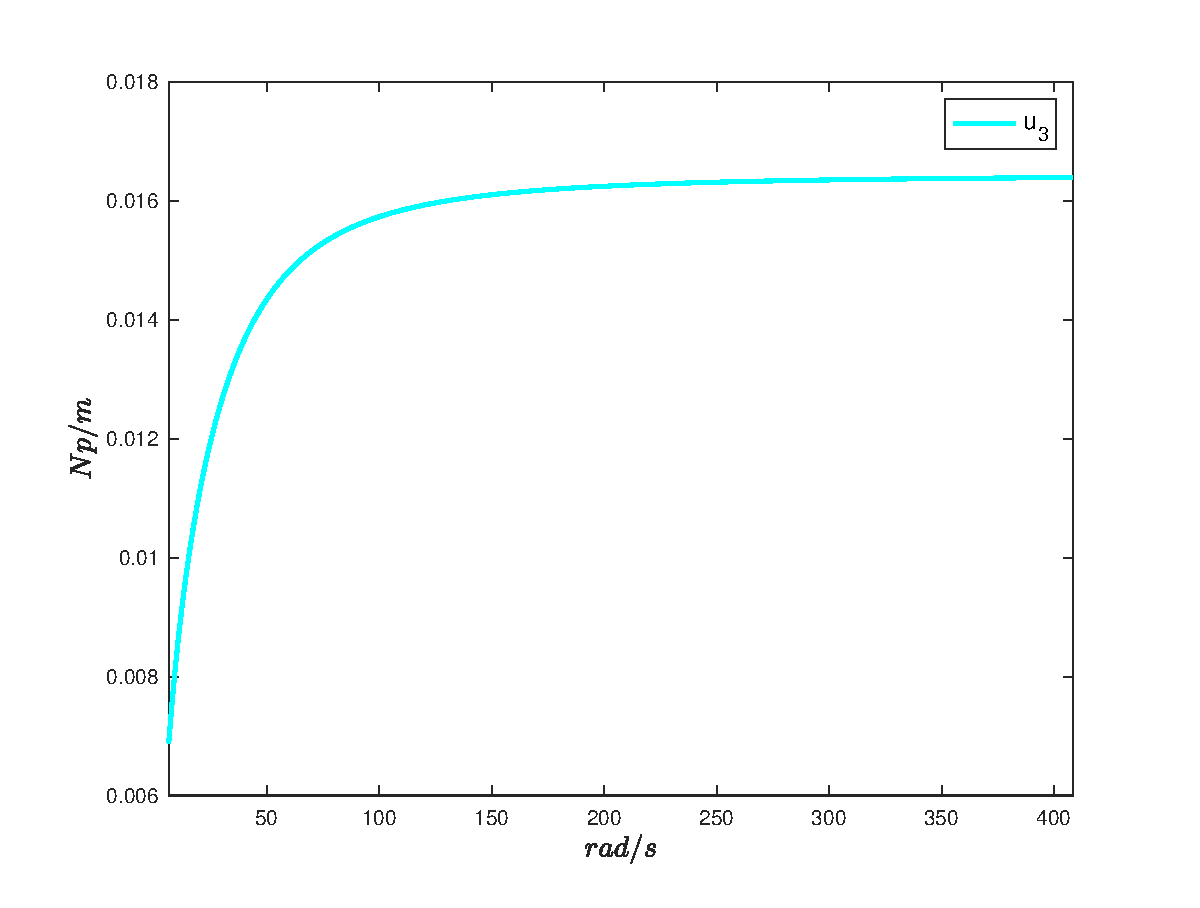
\includegraphics[scale=.43]{attenuation_ampere}}\\
\subfloat{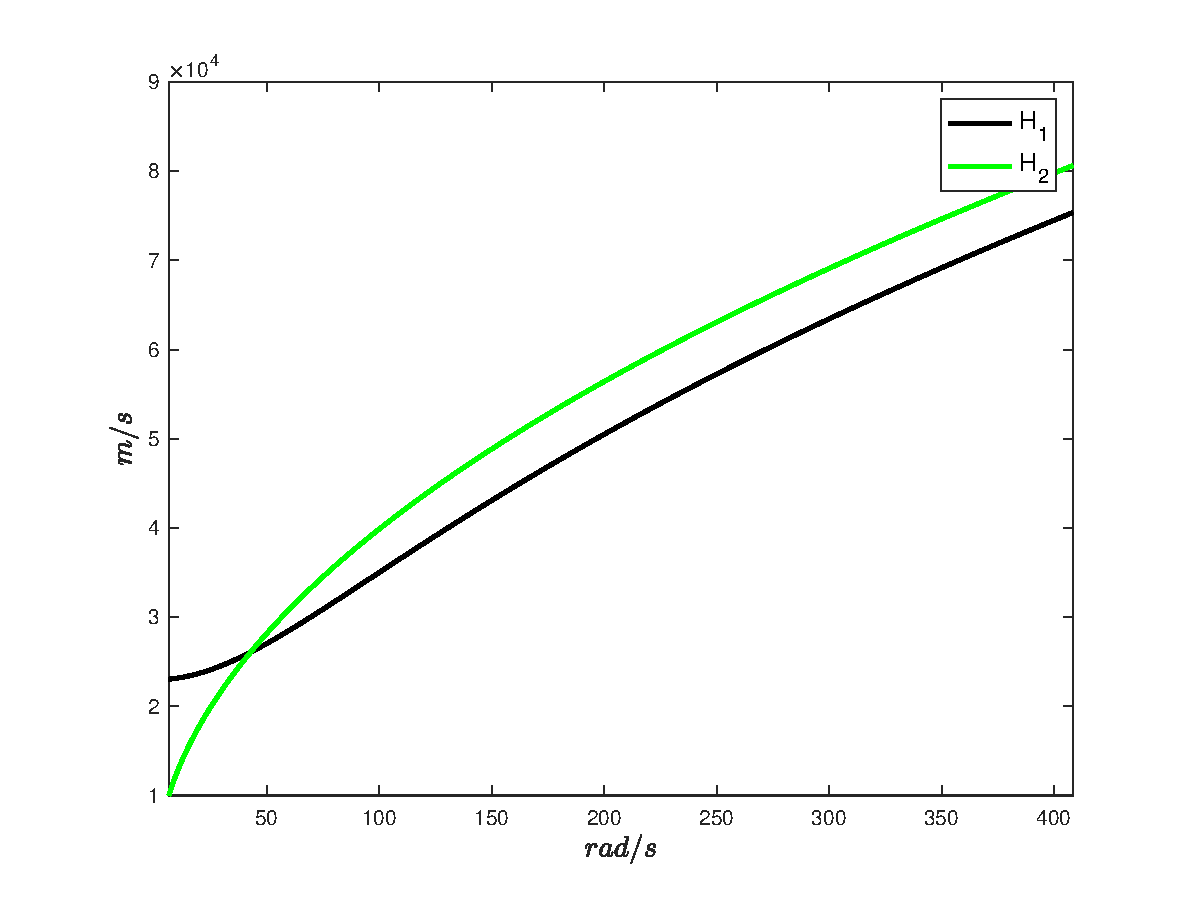
\includegraphics[scale=.43]{phase_veloc_ampere_3}}
\subfloat{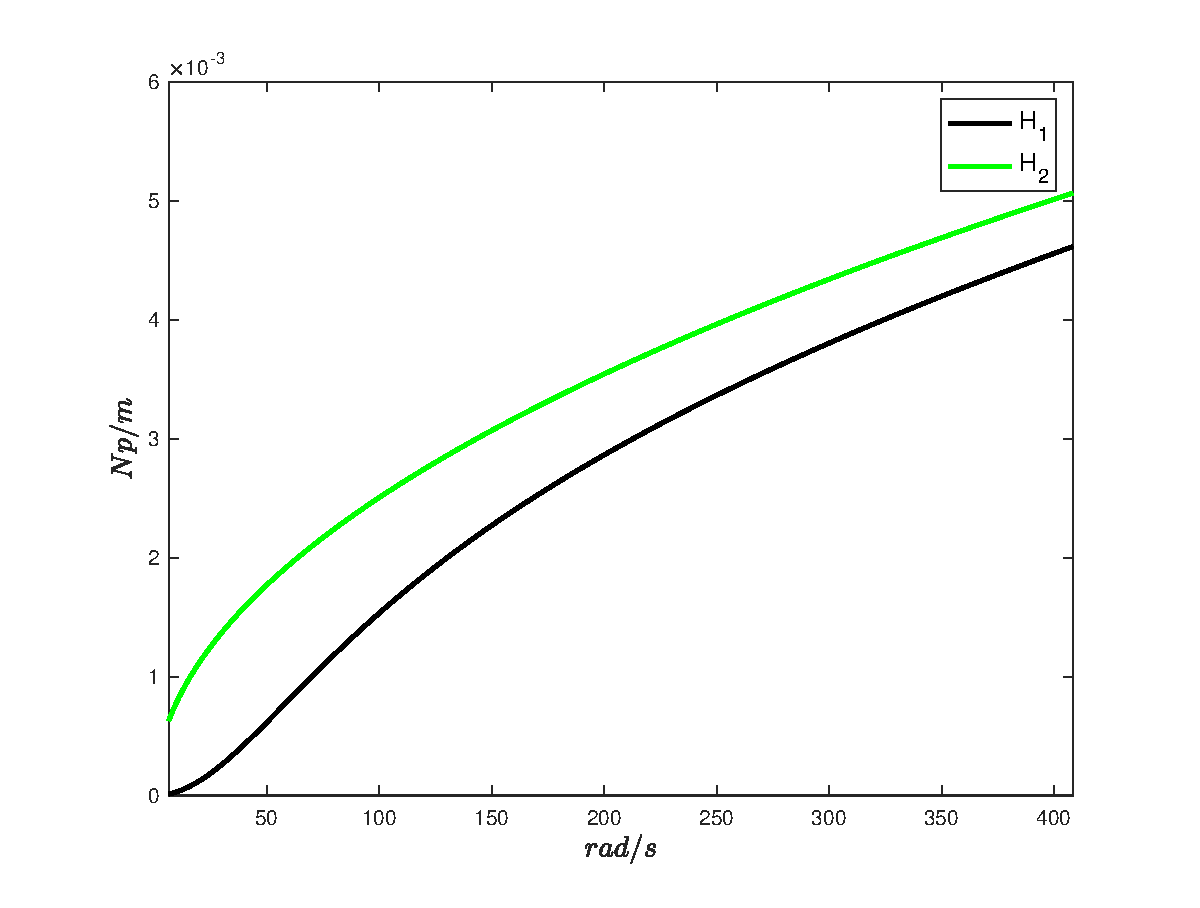
\includegraphics[scale=.43]{attenuation_ampere_3}}\\
%\subfloat{\includegraphics[scale=.57]{phase_veloc_ampere_5}}
%\subfloat{\includegraphics[scale=.57]{attenuation_ampere_5}}
\caption{\textit{Velocidade de fase e atenua\c{c}\~ao da onda el\'astica e de duas ondas eletromagn\'eticas em fun\c{c}\~ao da frequ\^encia angular e de um campo magn\'etico externo. Caso Amp\`ere-Maxwell.}}
\label{fig.disp_am_ma}
\end{figure}


\section{Caso An\'alogo \`a Lei de Faraday}\label{sec.faraday}

Pela lei de Faraday dada pela equa\c{c}\~ao (\ref{eq.faraday}), a varia\c{c}\~ao no tempo de um campo magn\'etico produz o rotacional de um campo el\'etrico que, consequentemente, produz o movimento de cargas el\'etricas num meio condutor. Para simularmos um efeito geometricamente an\'alogo \`a lei de Faraday, partindo das equa\c{c}\~oes (\ref{eq.disp_abertas_1}) e (\ref{eq.disp_abertas_2}), vamos considerar as duas primeiras componentes do campo el\'astico e a terceira componente do campo magn\'etico, se propagando no tempo e nas vari\'aveis $x$ e $y$. Desprezando a permissividade el\'etrica ainda como consequ\^encia do regime \textit{quasi}-estacion\'ario das equa\c{c}\~oes de Maxwell, temos o seguinte sistema
\begin{align*}
\rho\,\frac{\partial^2u_1}{\partial t^2}&=(\lambda+2G)\frac{\partial^2u_1}{\partial x^2}+(\lambda+G)\frac{\partial^2u_2}{\partial x\,\partial y}+G\frac{\partial^2u_1}{\partial y^2}-\mu_0H^0_3\frac{\partial H_3}{\partial x}\\\\
\rho\,\frac{\partial^2u_2}{\partial t^2}&=(\lambda+2G)\frac{\partial^2u_2}{\partial y^2}+(\lambda+G)\frac{\partial^2u_1}{\partial x\,\partial y}+G\frac{\partial^2u_2}{\partial x^2}-\mu_0H^0_3\frac{\partial H_3}{\partial y}\\\\
\frac{\partial H_3}{\partial t}&=V_H\left(\frac{\partial^2 H_3}{\partial x^2} +  \frac{\partial^2 H_3}{\partial y^2}\right) - H^0_3 \left(\frac{\partial^2 u_1}{\partial x \partial t} + \frac{\partial^2 u_2}{\partial y \partial t}\right).
\end{align*}
Aplicando as solu\c{c}\~oes em ondas planas dadas pelas equa\c{c}\~oes (\ref{eq.ondas_planas}), escrevendo os n\'umeros de ondas em termos de sua norma e dire\c{c}\~ao e agrupando as parcelas de acordo com as polariza\c{c}\~oes, temos o sistema alg\'ebrico homog\^eneo
\begin{align*}
\left[(\lambda+2G)\cos^2\theta k^2-\rho\omega^2+G\text{sen}^2\theta k^2\right]u_{01}+(\lambda+G)\text{sen}\theta\cos\theta k^2u_{02}-i\mu_0H^0_3\cos\theta kH_{03}&=0\\
(\lambda+G)\text{sen}\theta\cos\theta k^2u_{01}+\left[(\lambda+2G)\text{sen}^2\theta k^2-\rho\omega^2+G\cos^2\theta k^2\right]u_{02}-i\mu_0H^0_3\text{sen}\theta kH_{03}&=0\\
\omega\,H^0_3\cos\theta\,k\,u_{01}+\omega\,H^0_3\text{sen}\theta\,k\,u_{02}+\left[i\,\omega+V_Hk^2\right]H_{03}&=0.
\end{align*}
Com esse sistema acima podemos escolher a dire\c{c}\~ao de propaga\c{c}\~ao, e se escolhemos a propaga\c{c}\~ao na dire\c{c}\~ao do eixo $x$ e calculamos uma solu\c{c}\~ao n\~ao trivial, obtemos as velocidades de fase e atenua\c{c}\~oes atrav\'es das equa\c{c}\~oes
\begin{align}\label{eq.disp_ate_faraday_2}
&G\,k^2-\omega^2\rho=0\qquad\text{ou}\\\label{eq.disp_ate_faraday_1}
&V_H(\lambda+2G)k^4+\left[i\omega(\lambda+2G)-\omega^2\rho\,V_H+i\,\omega\,\mu_0(H_3^0)^2\right]k^2-i\,\omega^3\rho=0.
\end{align}
Note que a equa\c{c}\~ao (\ref{eq.disp_amp_max}) \'e muito parecida com a equa\c{c}\~ao (\ref{eq.disp_ate_faraday_1}), elas possuem basicamente duas diferen\c{c}as. Algebricamente, elas diferem pelo fato de que a equa\c{c}\~ao (\ref{eq.disp_amp_max}) est\'a escrita em fun\c{c}\~ao da magnitude do campo magn\'etico externo e a equa\c{c}\~ao (\ref{eq.disp_ate_faraday_1}) est\'a escrita em fun\c{c}\~ao da terceira componente do campo magn\'etico externo. Conceitualmente, a equa\c{c}\~ao (\ref{eq.disp_amp_max}) nos permite calcular a velocidade de fase e atenua\c{c}\~ao relacionadas \`as componentes $u_{3}$ e $H_{1}$ como foi visto, mas a equa\c{c}\~ao (\ref{eq.disp_ate_faraday_1}) nos permite calcular a velocidade de fase e atenua\c{c}\~ao relacionadas \`as componentes $u_{1}$ e $H_{3}$. A equa\c{c}\~ao (\ref{eq.disp_ate_faraday_2}) nos permite calcular a velocidade de fase e atenua\c{c}\~ao relacionada \`a a componente $u_{2}$, a qual se trata de uma onda transversal como podemos verificar algebricamente. Esse \'e o primeiro caso onde aparece propaga\c{c}\~ao de onda transversal, j\'a que agora estamos trabalhando com propaga\c{c}\~ao em duas dimens\~oes. Poder\'iamos escolher a propaga\c{c}\~ao na dire\c{c}\~ao do eixo $y$, mas desse jeito obtemos o mesmo sistema dado pelas equa\c{c}\~oes (\ref{eq.disp_ate_faraday_2}) e (\ref{eq.disp_ate_faraday_1}), com a \'unica diferen\c{c}a de que a onda longitudinal \'e que estaria relacionada \`a componente $u_{2}$ e a onda transversal \`a componente $u_{1}$, mas as caracter\'isticas dessas ondas n\~ao seriam alteradas. A equa\c{c}\~ao (\ref{eq.disp_ate_faraday_1}) pode ser resolvida com a abordagem descrita na subse\c{c}\~ao (\ref{sec.dispesion_1D}), mas dessa vez preferimos usar a ferramenta \textit{root} do \textit{MATLAB} que demonstrou um bom funcionamento, boa velocidade e confec\c{c}\~ao dos gr\'aficos.

Na figura \ref{fig.disp_fa_x_dir} podemos observar a velocidade de fase e atenua\c{c}\~ao considerando a propaga\c{c}\~ao na dire\c{c}\~ao do eixo $x$, utilizando as equa\c{c}\~oes \ref{eq.disp_ate_faraday_2}
 e \ref{eq.disp_ate_faraday_1}. Com excess\~ao da onda $S$, note que os gr\'aficos se mant\^em similares aos anteriores mesmo utilizando a terceira componente do campo magn\'etico externo no lugar da magnitude horizontal do campo magn\'etico externo. A velocidade da onda transversal \'e constante e vale 1200 $m/s$, o que \'e equivalente a aproximadamente $60\%$ da velocidade da onda longitudinal que varia com a frequ\^encia e chega a 2000 $m/s$. Apesar do comportamento comum da atenua\c{c}\~ao da onda longitudinal, a atenua\c{c}\~ao da onda transversal \'e identicamente nula pois o n\'umero de onda da onda $S$  possui valor real em nosso modelo, ou seja, temos um caso n\~ao atenuativo. Novamente, a velocidade da onda eletromagn\'etica varia com a frequ\^encia e \'e bem menor que sua velocidade no v\'acuo, como consequ\^encia da pouca influ\^encia que a permissividade el\'etrica tem em nosso modelo. O campo magn\'etico externo, mesmo sendo aplicado com muito mais for\c{c}a que o campo geomagn\'etico, n\~ao parece afetar significativamente a velocidade e atenua\c{c}\~ao das ondas mec\^anicas, da mesma forma que n\~ao afetou para os dois modelos anteriores.
 
\begin{figure}
\centering
\subfloat{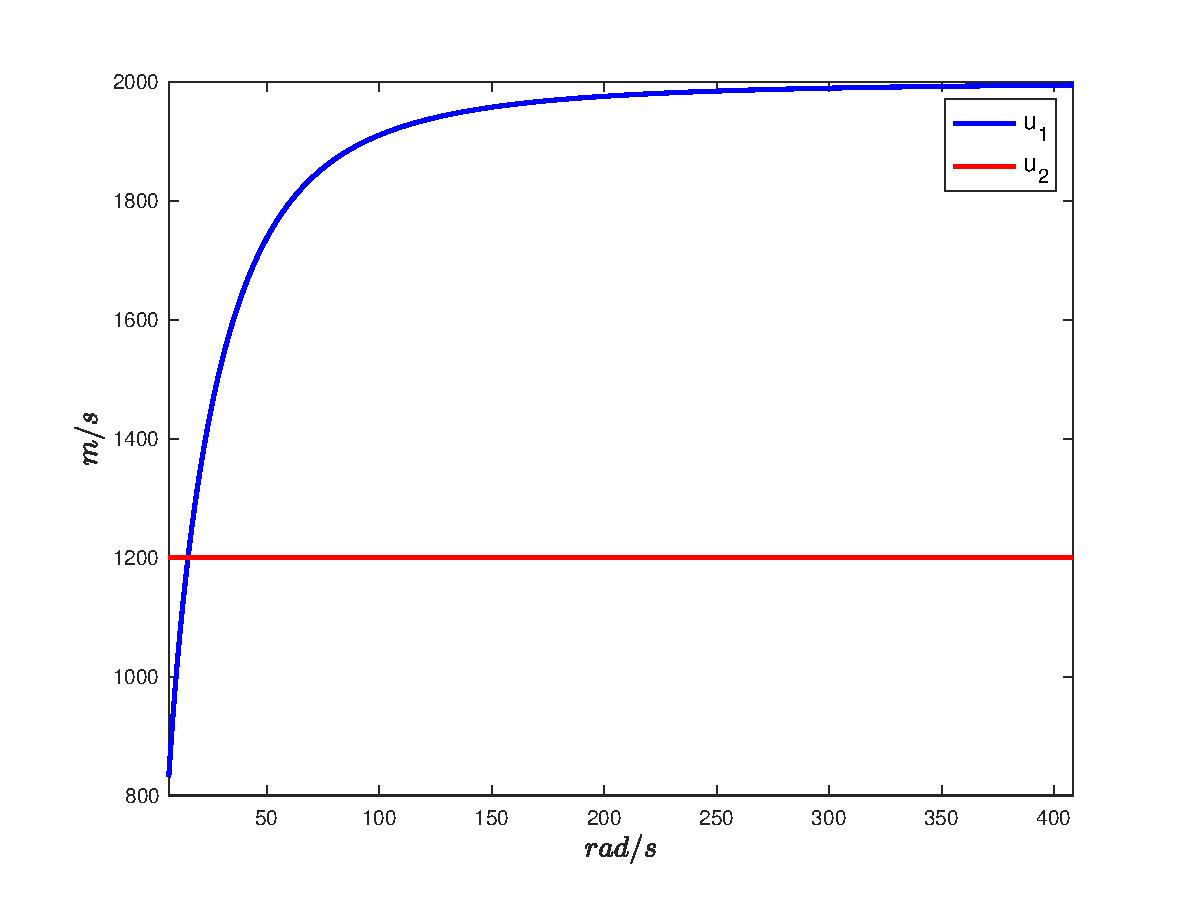
\includegraphics[scale=.425]{pha_vel_fara_x_dir}}
\subfloat{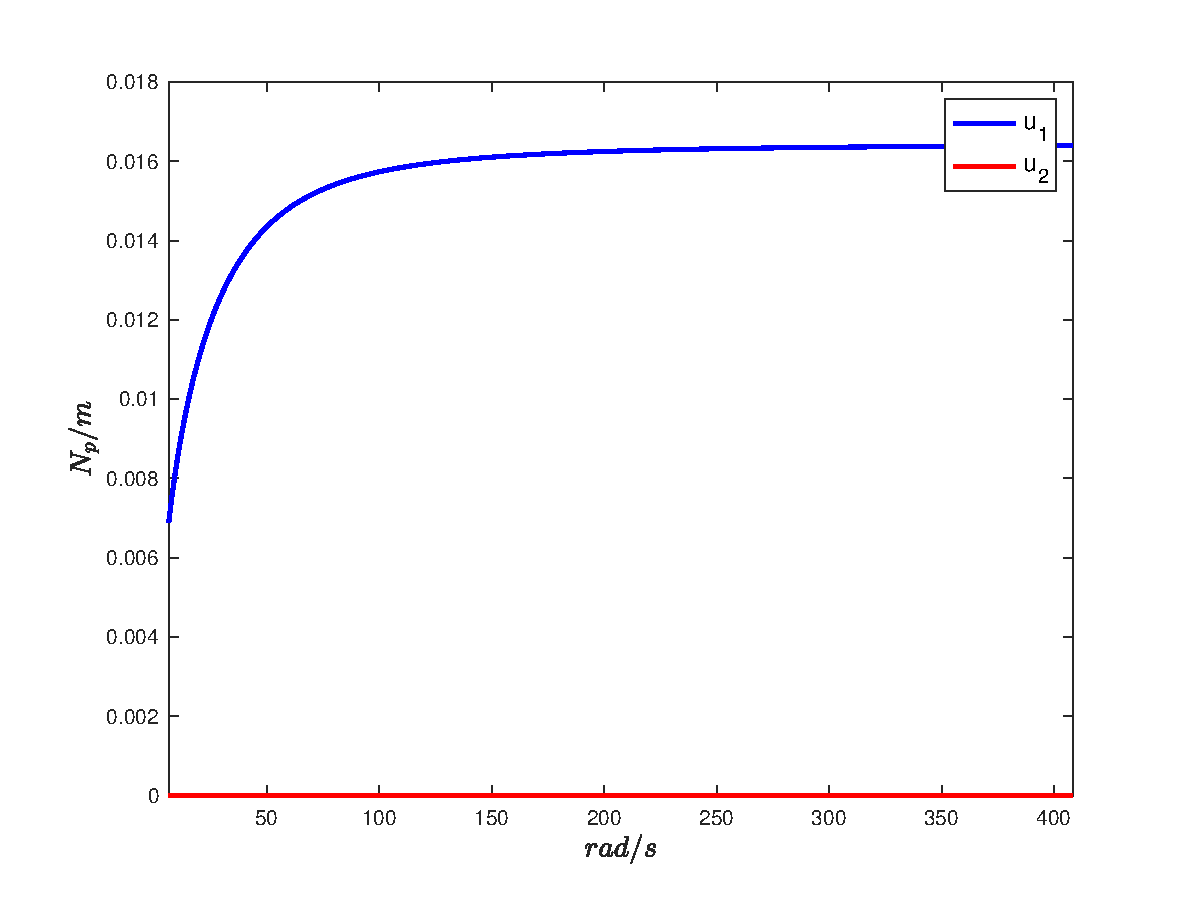
\includegraphics[scale=.425]{atte_u_fara_x_direc}}\\
%\subfloat{\includegraphics[scale=.57]{phase_veloc_faraday_3}}
%\subfloat{\includegraphics[scale=.57]{attenuation_faraday_3}}\\
\subfloat{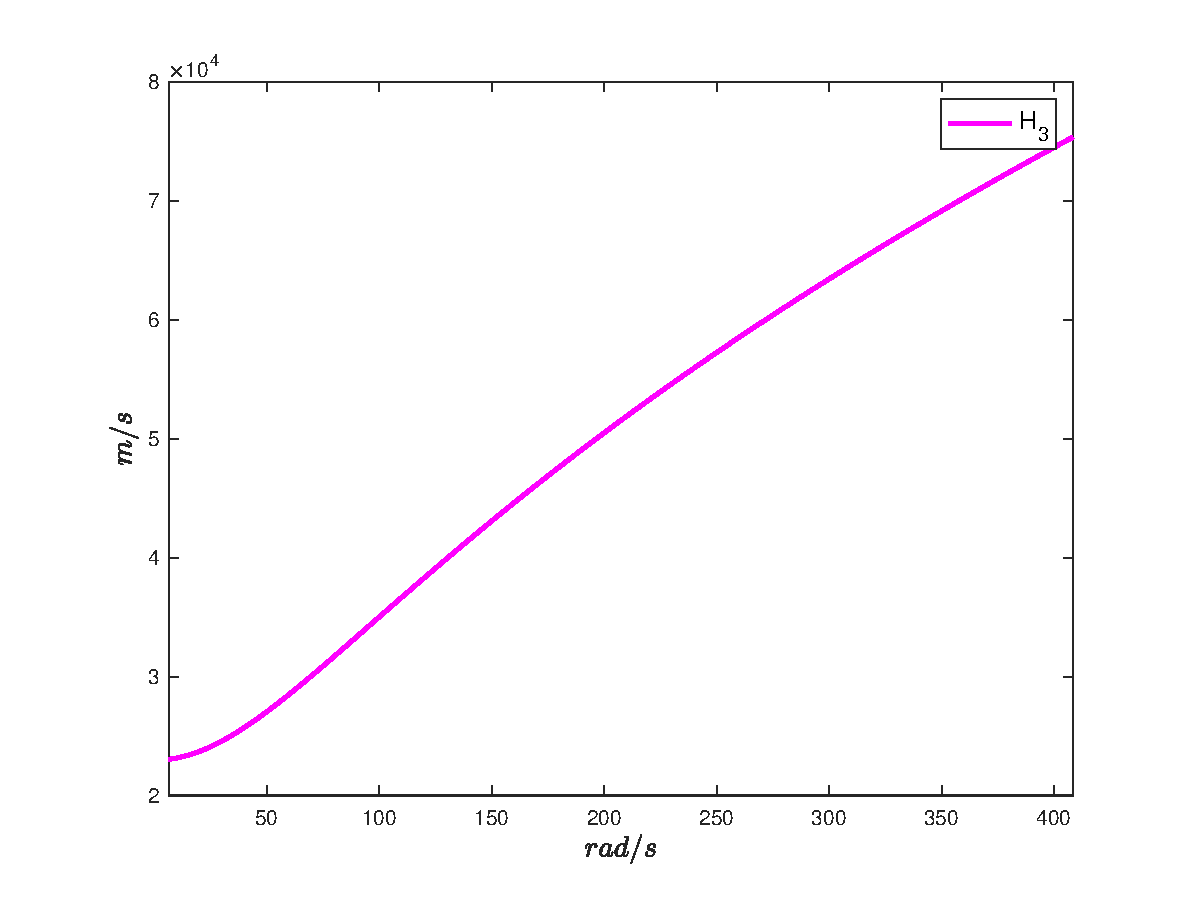
\includegraphics[scale=.425]{pha_vel_H_fara_x_dir}}
\subfloat{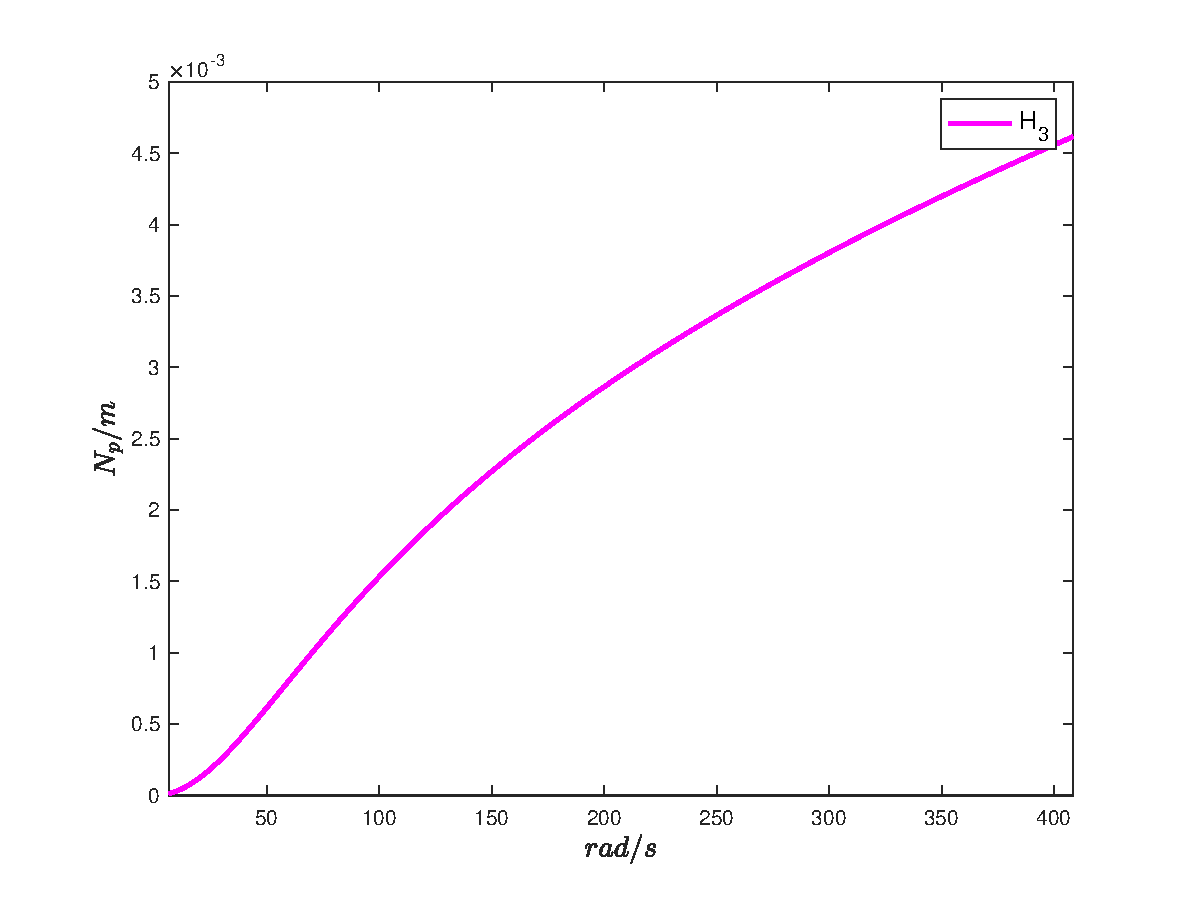
\includegraphics[scale=.425]{att_H_fara_x_direc}}
\caption{\textit{Velocidade de fase e atenua\c{c}\~ao de duas ondas el\'asticas e de uma onda eletromagn\'etica, que se propagam na dire\c{c}\~ao do eixo $x$, e em fun\c{c}\~ao da frequ\^encia angular e de um campo magn\'etico externo. Caso Faraday.}}
\label{fig.disp_fa_x_dir}
\end{figure}

Para promovermos a propaga\c{c}\~ao das ondas numa dire\c{c}\~ao qualquer do espa\c{c}o horizontal n\~ao podemos usar as equa\c{c}\~oes  \ref{eq.disp_ate_faraday_2} e \ref{eq.disp_ate_faraday_1}, devemos escolher a dire\c{c}\~ao atrav\'es do \^angulo $\theta$ no sistema acima. Buscando por uma solu\c{c}\~ao n\~ao trivial desse sistema, encontramos uma equa\c{c}\~ao polinomial de grau 6, j\'a que n\~ao \'e mais poss\'ivel separar quaisquer das equa\c{c}\~oes do sistema. Usando a ferramenta \textit{root} para extrair as seis ra\'izes, n\~ao obtivemos boa confec\c{c}\~ao dos gr\'aficos. Para contornar o problema, fatoramos o quadrado do n\'umero de onda e transformamos o polin\^omio para grau 3, o qual n\~ao foi bem resolvido usando as f\'ormulas para polin\^omios de terceiro grau encontradas em \cite{abramovitz_64}. Essas f\'ormulas funcionaram bem em testes com coeficientes inteiros, mas n\~ao com os coeficientes do nosso problema, possivelmente porque essas f\'ormulas requerem o uso da ferramenta \textit{sqrt} diversas vezes, o que pode estar prejudicando a precis\~ao das ra\'izes. Uma aboradgem que trouxe resultados um pouco mais satisfat\'orios foi utilizar a ferramenta \textit{root} para extrair as tr\^es ra\'izes e em seguida utilizar a ferramenta \textit{root} apenas uma vez em cada uma das ra\'izes. Os gr\'aficos usando $\theta=\frac{\pi}{4}\,rad$ podem ser visualizados no ap\^endice (\ref{sec.app_faraday}) e n\~ao ficaram plenamente bons, mas ficaram bem parecidos com os gr\'aficos da figura (\ref{fig.disp_fa_x_dir}), sugerindo que n\~ao importa a dire\c{c}\~ao de propaga\c{c}\~ao das ondas no c\'alculo da velocidade de fase e atenua\c{c}\~ao. Tal resultado pode ser consequ\^encia de estarmos trabalhando com meios homog\^eneos e isotr\'opicos.

At\'e aqui temos aplicado um campo magn\'etico externo bastante forte mas com condutividade t\'ipica de camada estratigr\'afica, como podemos verificar na tabela (\ref{tab.dados_dispersao}), e tal abordagem n\~ao parece ter influ\^encia significativa sobre as ondas do efeito magneto-el\'astico. Aumentando tamb\'em a condutividade, aumentamos a intera\c{c}\~ao entre o meio de propaga\c{c}\~ao das ondas e o campo magn\'etico externo, e assim provocamos altera\c{c}\~oes na velocidade de propaga\c{c}\~ao dessas ondas. Para observarmos essas altera\c{c}\~oes, simulamos a propaga\c{c}\~ao na dire\c{c}\~ao do eixo $x$ usando condutividades at\'ipicas de $1\,S/m$ e $10\,S/m$ e, \`a medida que a condutividade \'e aumentada, h\'a redu\c{c}\~ao na velocidade da onda longitudinal, e a velocidade da onda eletromagn\'etica parece se tornar constante. Podemos conjecturar que, quando aumentamos a condutividade do meio, aumentamos a for\c{c}a de atra\c{c}\~ao entre o mesmo e o campo magn\'etico externo, que tamb\'em \'e muito forte. Com o meio sofrendo essa forte atra\c{c}\~ao, pode ser que sua capacidade de oscila\c{c}\~ao ou suas caracter\'isticas el\'asticas sejam alteradas, provocando a diminui\c{c}\~ao na velocidade da onda mec\^anica longitudinal. A velocidade da onda transversal n\~ao foi alterada, como era de se esperar quando analisamos a equa\c{c}\~ao (\ref{eq.disp_ate_faraday_2}), provavelmente devido \`as hip\'oteses simplificadoras do modelo. Podemos analisar os gr\'aficos das velocidades das ondas para altas condutividades na figura (\ref{fig.disp_fa_x_sig}), e ver que a velocidade da onda longitudinal \'e reduzida para aproximadamente 700 $m/s$ em altas frequ\^encias, e que praticamente n\~ao h\'a varia\c{c}\~ao na velocidade da onda eletromagn\'etica. 

\begin{figure}
\centering
\subfloat{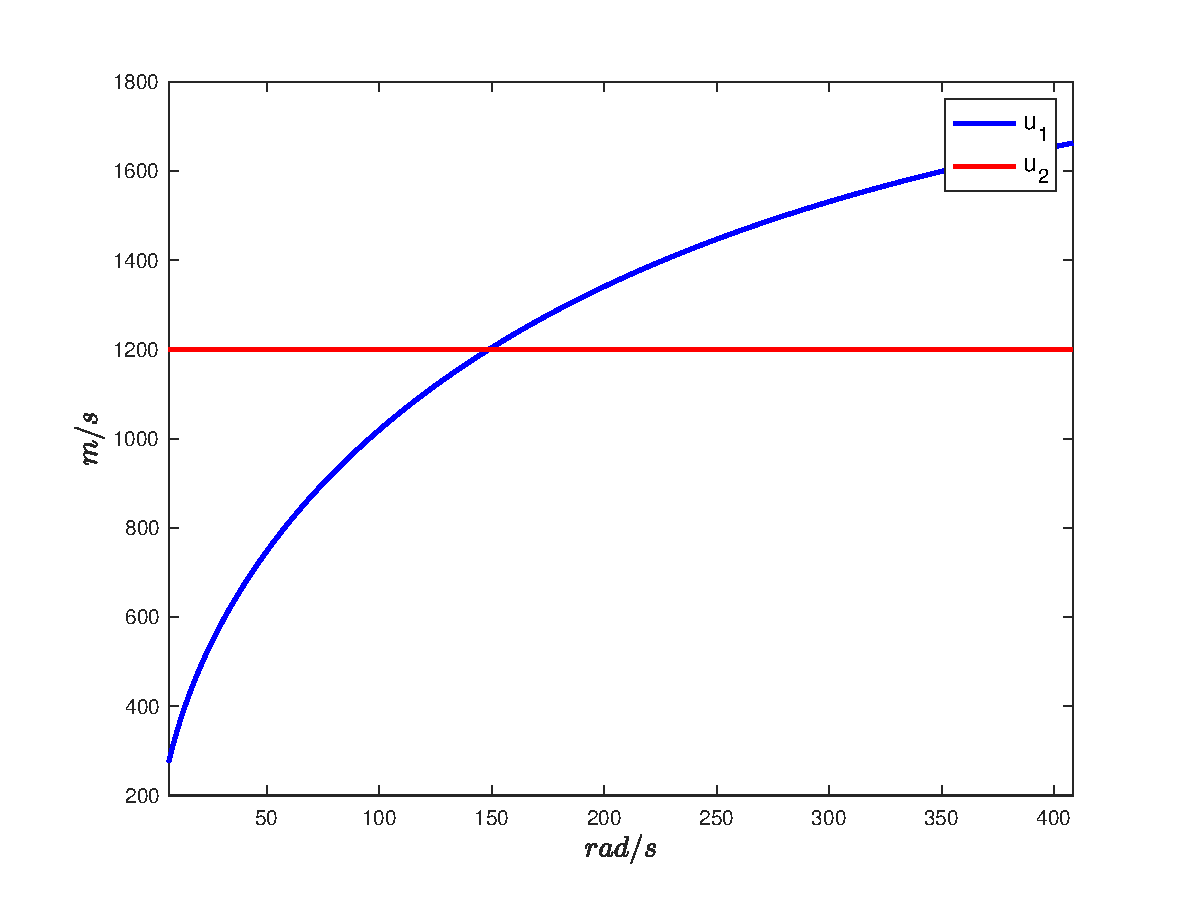
\includegraphics[scale=.425]{u_far_sig_1}}
\subfloat{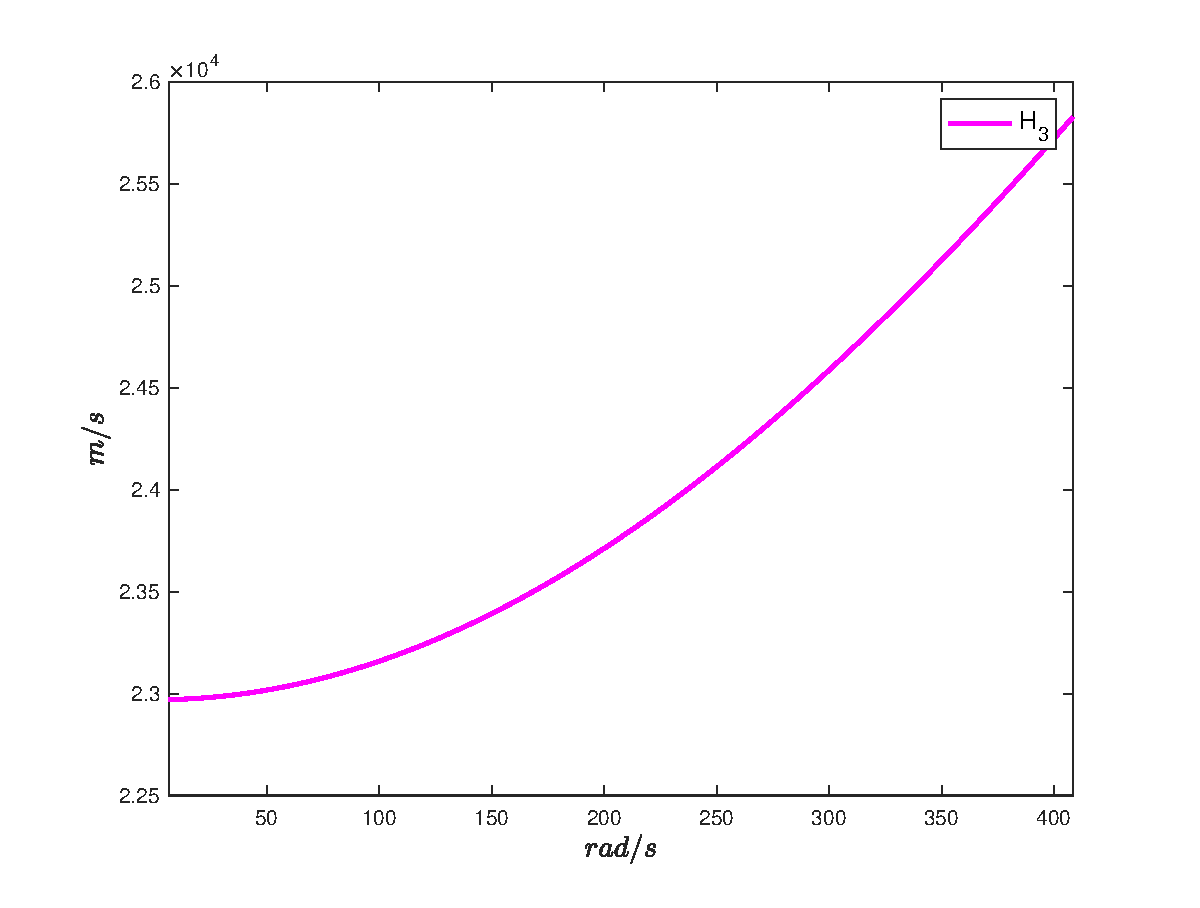
\includegraphics[scale=.425]{h_far_sig_1}}\\
%\subfloat{\includegraphics[scale=.57]{phase_veloc_faraday_3}}
%\subfloat{\includegraphics[scale=.57]{attenuation_faraday_3}}\\
\subfloat{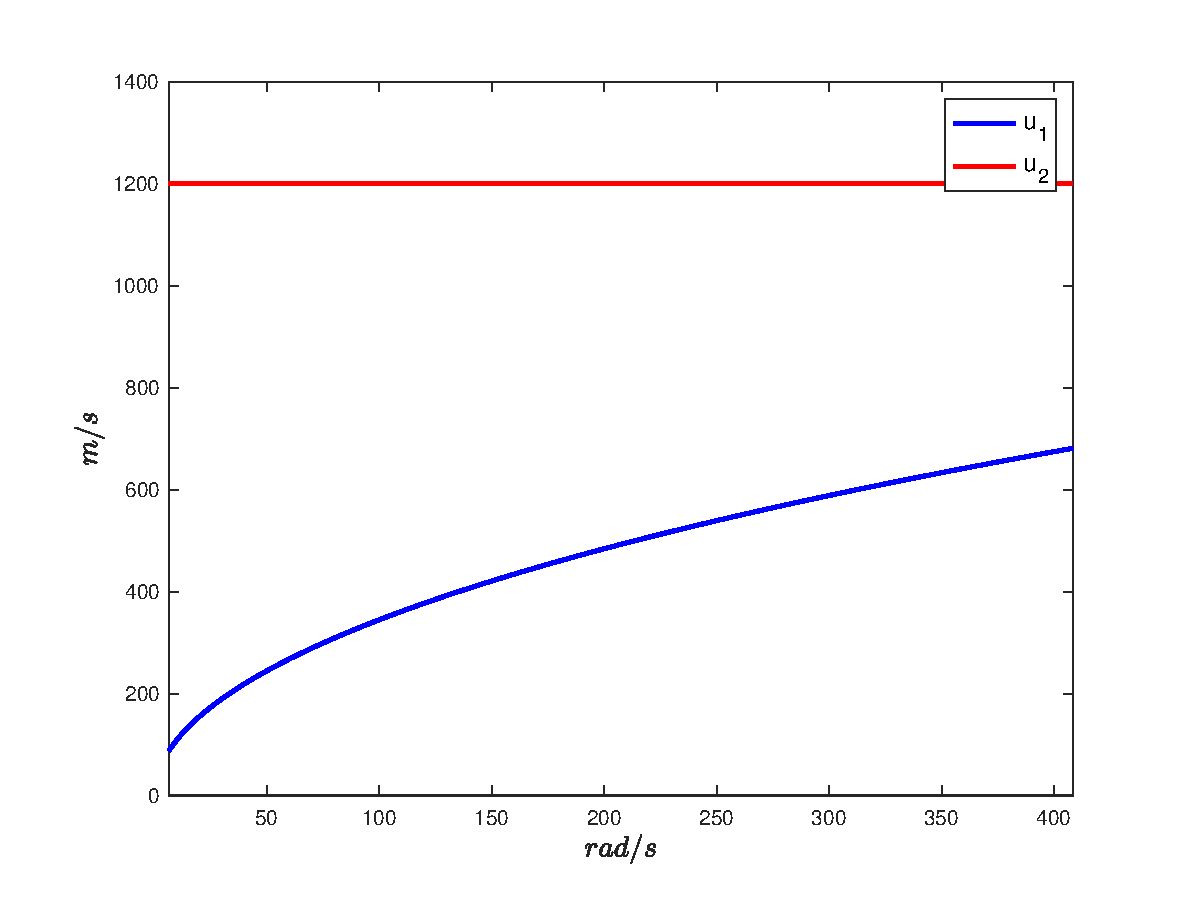
\includegraphics[scale=.425]{u_far_sig_10}}
\subfloat{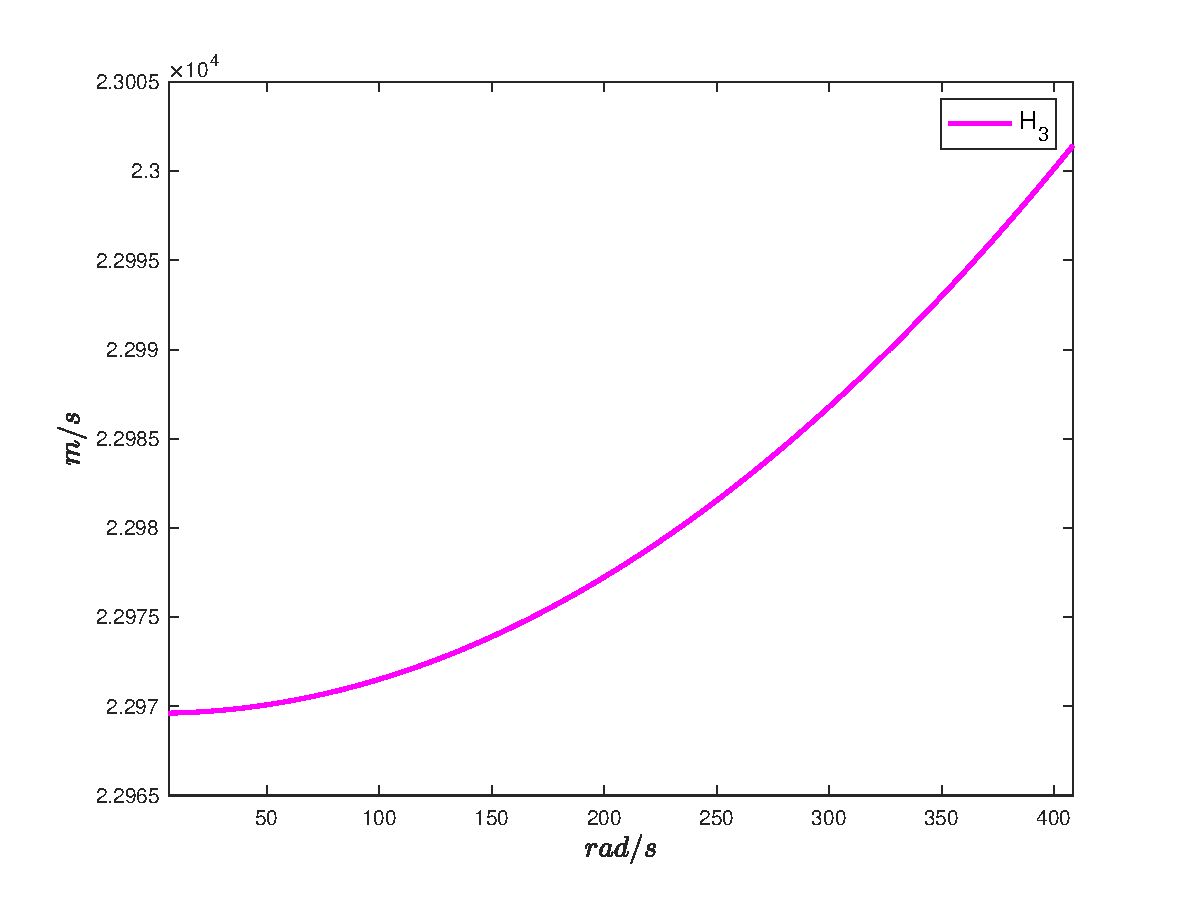
\includegraphics[scale=.425]{h_far_sig_10}}
\caption{\textit{Nos dois gr\'aficos de cima temos as velocidades considerando $\sigma=1\,S/m$ e nos gr\'aficos de baixo $\sigma=10\,S/m$.}}
\label{fig.disp_fa_x_sig}
\end{figure}

%
% Na figura (\ref{fig.disp_fa}) temos os gr\'aficos mostrando as velocidades de fase e atenua\c{c}\~oes para os dois campos mec\^anicos e para o campo eletromagn\'etico, e diferentemente do constatado para os dois campos magn\'eticos do caso Amp\`ere-Maxwell na subse\c{c}\~ao (\ref{sec.ampere_maxwell_law}), aqui temos comportamentos expressivamente diferentes para os dois campos mec\^anicos. Para frequ\^encias acima de 200 $rad/s$, a velocidade usando a polariza\c{c}\~ao $u_{01}$ \'e menor que da polariza\c{c}\~ao $u_{02}$ e essa diferen\c{c}a chega a aproximadamente 600 $m/s$ quando a frequ\^encia \'e  400 $rad/s$. Tal fato sugere que $u_{01}$ representa a velocidade de uma onda transversal e $u_{02}$ representa a velocidade de uma onda longitudinal. Al\'em disso, observando o gr\'afico de atenua\c{c}\~ao nessa mesma figura, temos que a atenua\c{c}\~ao usando a polariza\c{c}\~ao $u_{01}$ \'e menor do que da polariza\c{c}\~ao $u_{02}$, ou seja, a amplitude da onda descrita por $u_{01}$ seria maior do que da onda descrita por $u_{02}$ sob mesmas condi\c{c}\~oes de propaga\c{c}\~ao. Podemos observar em sismogramas que a amplitude de ondas transversais podem ser maiores do que de ondas longitudinais, e essa diferen\c{c}a de amplitudes tamb\'em pode ser observada nos eventos 2 e 3 das figuras (\ref{fig.v3}) e (\ref{fig.v3_750}). Portanto, esse fato pode ser mais um ind\'icio de que $u_{01}$ descreva uma onda transversal e $u_{02}$ descreva uma onda longitudinal.  
%
%\begin{figure}
%\centering
%\subfloat{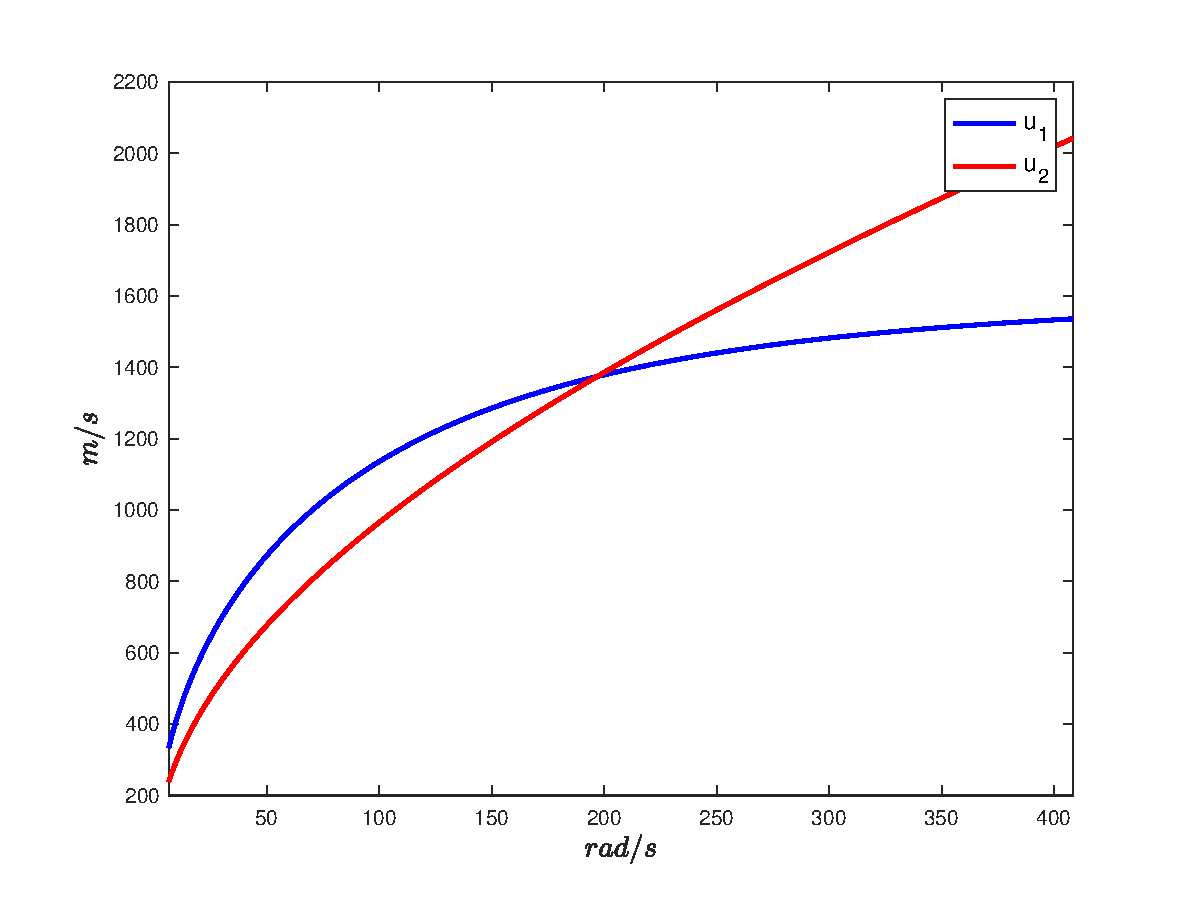
\includegraphics[scale=.43]{phase_veloc_faraday}}
%\subfloat{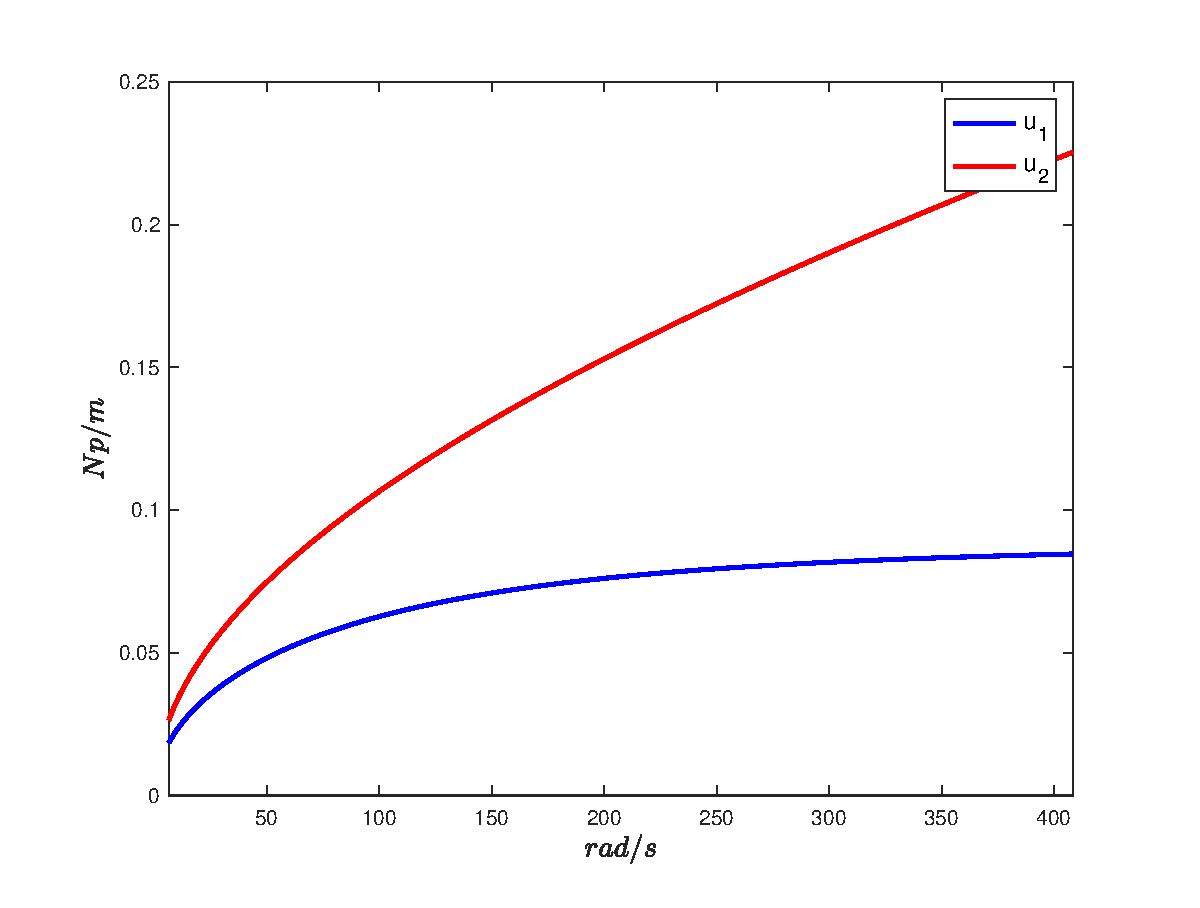
\includegraphics[scale=.43]{attenuation_faraday}}\\
%%\subfloat{\includegraphics[scale=.57]{phase_veloc_faraday_3}}
%%\subfloat{\includegraphics[scale=.57]{attenuation_faraday_3}}\\
%\subfloat{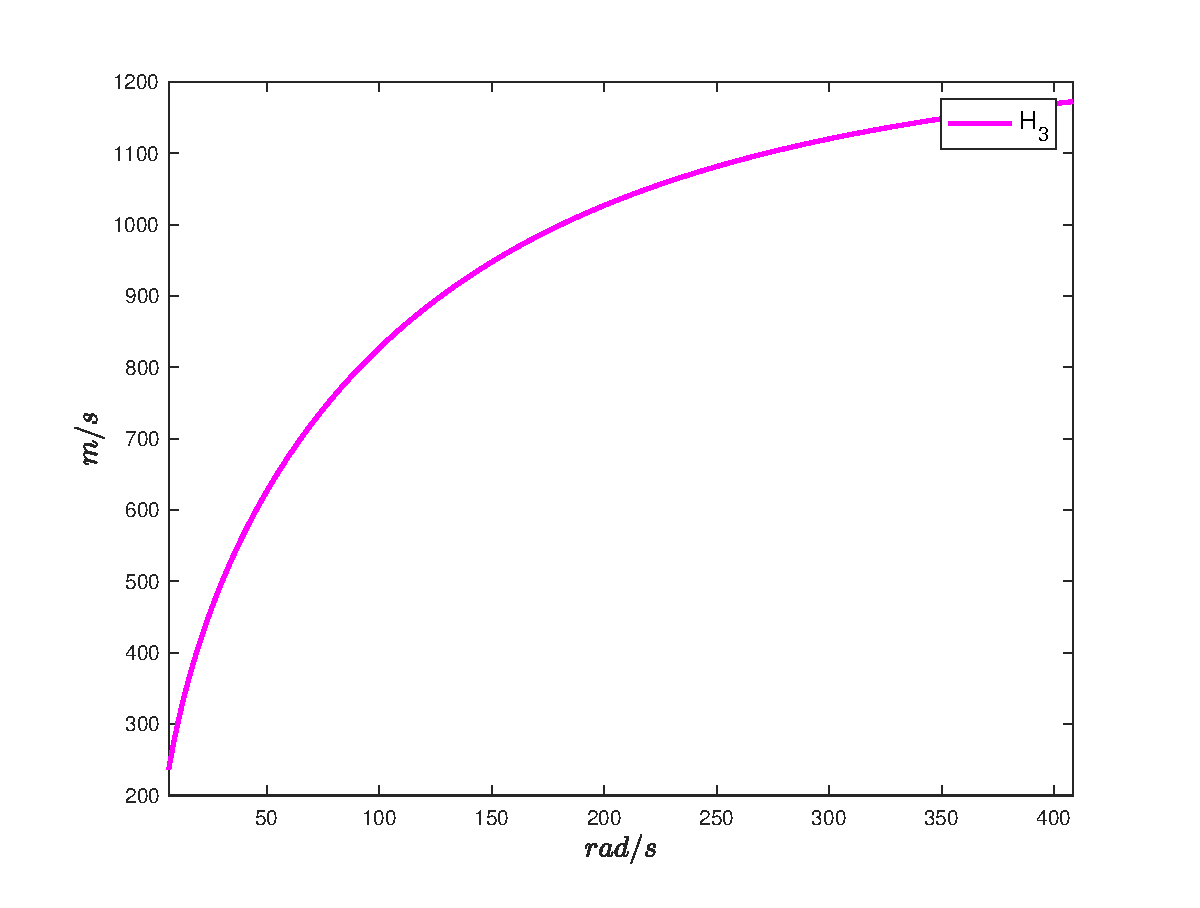
\includegraphics[scale=.43]{phase_veloc_faraday_5}}
%\subfloat{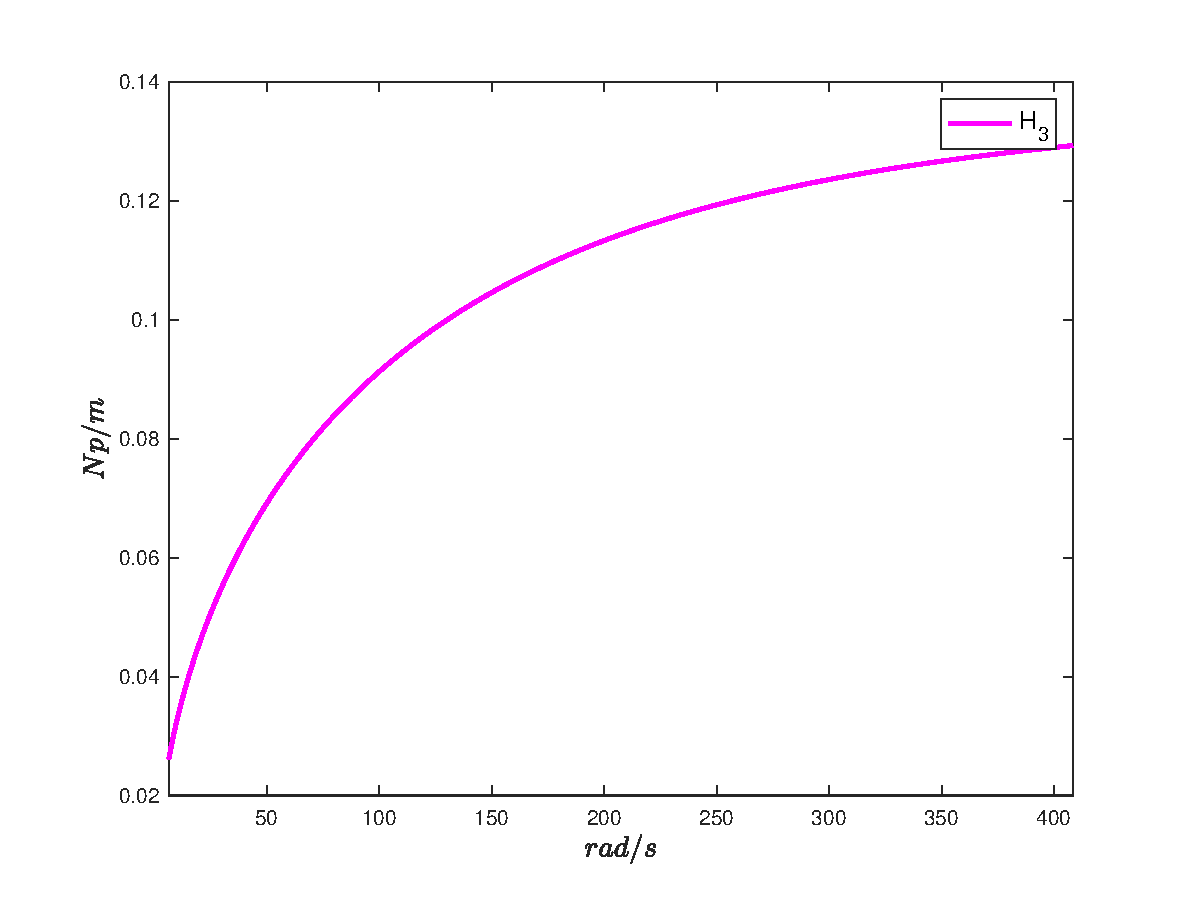
\includegraphics[scale=.43]{attenuation_faraday_5}}
%\caption{\textit{Velocidade de fase e atenua\c{c}\~ao de duas ondas el\'asticas e de uma onda eletromagn\'etica, em fun\c{c}\~ao da frequ\^encia angular e de um campo magn\'etico externo. Caso Faraday.}}
%\label{fig.disp_fa}
%\end{figure}


% FORMA MATRICIAL DO SISTEMA ACIMA (PROBLEMA DE ESPACO)
%\begin{equation}
%\begin{pmatrix}
%-(\lambda+2G)\cos^2\theta\,k^2+\rho\,\omega^2-G\,\text{sen}^2\theta\,k^2&-(\lambda+G)\text{sen}\theta\cos\theta\,k^2&i\,\mu_0H^0_3\cos\theta\,k\\
%-(\lambda+G)\text{sen}\theta\cos\theta\,k^2&-(\lambda+2G)\text{sen}^2\theta\,k^2+\rho\,\omega^2-G\,\cos^2\theta\,k^2&i\,\mu_0H^0_3\text{sen}\theta\,k\\
%
%\end{pmatrix}
%\begin{pmatrix}
%u_{01}\\
%u_{02}\\
%H_{03}
%\end{pmatrix}
%=
%\begin{pmatrix}
%0\\
%0\\
%0
%\end{pmatrix}
%\end{equation}

\section{Campo Magn\'etico Externo e Viscosidade Magn\'etica Nulos}

Partindo novamente das equa\c{c}\~oes (\ref{eq.disp_abertas_1}) e (\ref{eq.disp_abertas_2}), podemos estudar um caso composto pelas tr\^es fun\c{c}\~oes el\'asticas e duas eletromagn\'eticas, no dom\'inio do tempo e da profundidade. Essa abordagem \'e interessante pois permite analisar, de forma mais clara,  tr\^es subcasos que s\~ao de interesse te\'orico. Sendo assim, considerando o regime \textit{quasi}-estacion\'ario das equa\c{c}\~oes de Maxwell com eletrocondutividade finita, vamos desconsiderar  o espa\c{c}o horizontal para obtermos as EDP's a serem estudadas. Observe que, com as ondas se propagando somente na profundidade, na lei de Faraday temos que $\frac{\partial H_3}{\partial t}=0$ e $H_3=H_3^0$ \'e uma constante. Desta forma, zeramos toda a equa\c{c}\~ao para a componente vertical do campo magn\'etico, e constru\'imos o sistema 
\begin{align}\label{eq.u1_time}
\rho\frac{\partial^2 u_1}{\partial t^2}&=G\,\frac{\partial^2 u_1}{\partial z^2}+\mu_0H_3^0\frac{\partial H_1}{\partial z}\\\nonumber\\\label{eq.u2_time}
\rho\frac{\partial^2 u_2}{\partial t^2}&=G\,\frac{\partial^2 u_2}{\partial z^2}+\mu_0H_3^0\frac{\partial H_2}{\partial z}\\\nonumber\\\label{eq.u3_time}
\rho\frac{\partial^2 u_3}{\partial t^2}&=(\lambda+2\,G)\frac{\partial^2 u_3}{\partial z^2}-\mu_0\left[H_2^0\frac{\partial H_2}{\partial z}+H_1^0\frac{\partial H_1}{\partial z} \right]\\\nonumber\\\label{eq.H1_time}
\frac{\partial H_1}{\partial t}&=V_H\frac{\partial^2 H_1}{\partial z^2}+H_3^0\frac{\partial^2 u_1}{\partial z\partial t}-H_1^0\frac{\partial^2 u_3}{\partial z\partial t}\\\nonumber\\\label{eq.H2_time}
\frac{\partial H_2}{\partial t}&=V_H\frac{\partial^2 H_2}{\partial z^2}+H_3^0\frac{\partial^2 u_2}{\partial z\partial t}-H_2^0\frac{\partial^2 u_3}{\partial z\partial t}.
\end{align}
DEFINE MONOCHROMATIC WAVE AT SOME POINT OF THE TEXT\\
Para proceder a an\'alise de dispers\~ao e atenua\c{c}\~ao em uma onda monocrom\'atica, vamos aplicar no sistema acima as solu\c{c}\~oes em ondas planas no formato dado pela equa\c{c}\~oes (\ref{eq.ondas_planas}). Substituindo as solu\c{c}\~oes em ondas planas no sistema acima, obtemos um sistema de equa\c{c}\~oes homogen\^eas cujo a matriz de coeficientes \'e dada por
\begin{equation*}
\begin{pmatrix}
-Gk^2+\rho\,\omega^2&0&0&-i\,\mu_0H^0_3k&0\\
0&-Gk^2+\rho\,\omega^2&0&0&-i\,\mu_0H^0_3k\\
0&0&-(\lambda+2G)k^2+\rho\,\omega^2&i\,\mu_0H^0_1k&i\,\mu_0H^0_2k\\
H^0_3k\,\omega&0&-H^0_1k\,\omega&-V_Hk^2-i\,\omega&0\\
0&H^0_3k\,\omega&-H^0_2k\,\omega&0&-V_Hk^2-i\,\omega
\end{pmatrix},
\end{equation*}
onde buscaremos novamente pela solu\c{c}\~ao n\~ao trivial.

\subsection{Subcaso $H_3^0=0$.}
Tomando a terceira componente do campo magn\'etico externo igual a zero, temos o desacoplamento da segunda e da primeira componentes do campo el\'astico com os campos eletromagn\'eticos, e essas ondas el\'asticas se propagam com velocidade constante $\sqrt{\frac{G}{\rho}}$. Para as demais ondas que permanecem no sistema, podemos realizar a an\'alise de dispers\~ao e atenua\c{c}\~ao. No entanto, repare que esse \'e o mesmo caso an\'alogo \`a lei de Amp\`ere-Maxwell j\'a estudado na subse\c{c}\~ao (\ref{sec.ampere_maxwell_law}). Sendo assim, vamos passar para o pr\'oximo subcaso.

\subsection{Subcaso $H_1^0=0$ e $H_2^0=0$.}

Com as duas primeiras componentes do campo magn\'etico externo iguais a zero, temos o desacoplamento da terceira componente do campo el\'astico, a qual se propaga com velocidade constante igual a $\sqrt{\frac{\lambda+2G}{\rho}}$. Podemos determinar a rela\c{c}\~ao de dispers\~ao para os demais campos, $u_1$, $u_2$, $H_1$ e $H_2$, a qual \'e dada por
\begin{equation}
(-Gk^2+\rho\,\omega^2)^2(-V_Hk^2-i\,\omega)^2+\mu_0^2(H_3^0)^4\omega^2k^4=0.
\end{equation}
Essa rela\c{c}\~ao \'e uma equa\c{c}\~ao polinomial de grau 8 no n\'umero de onda, cujas ra\'izes nos fornecem a velocidade e atenua\c{c}\~ao. A ferramenta \textit{root} que n\~ao funciona muito bem em casos anteriores e de menor complexidade, tamb\'em n\~ao \'e eficiente aqui. A estrat\'egia de fatorar o quadrado do n\'umero de onda e determinar as ra\'izes de um polin\^omio de quarto grau tamb\'em n\~ao produz solu\c{c}\~oes com a acur\'acia necess\'aria usando essa ferramenta. Em \cite{abramovitz_64}, encontramos um m\'etodo anal\'itico para c\'alculo das ra\'izes de polin\^omio de quarto grau, que se baseia no c\'alculo das ra\'izes de um polin\^omio de grau tr\^es obtido a partir do polin\^omio original de grau quatro, mas tamb\'em sem sucesso. Assim, aplicamos outra ferramenta que n\~ao est\'a no pacote b\'asico do \textit{MATLAB} chamada \textit{vpasolve}, e que pode ser encontrada no pacote \textit{Symbolic Math Toolbox}. Enquanto que usando as abordagens num\'ericas dos casos anteriores o tempo de execu\c{c}\~ao era de segundos, usando \textit{vpasolve} o tempo \'e de horas. Como precisavamos de muitas execu\c{c}\~oes at\'e acertar o c\'odigo, diminu\'imos bastante o passo de frequ\^encia para reduzir o tempo de execu\c{c}\~ao. Depois de ajustado o c\'odigo, executamos com o mesmo passo de frequ\^encia dos casos anteriores para obter os gr\'aficos da figura (\ref{fig.mag_horiz_ext_nula}).

Analisando os gr\'aficos percebemos que n\~ao houve altera\c{c}\~oes muito discrepantes em rela\c{c}\~ao aos tr\^es casos anteriores e todas as componentes continuam com valores na ordem de grandeza esperada. Apesar da varia\c{c}\~ao mostrada no gr\'afico, a velocidade de fase e atenua\c{c}\~ao relacionadas \`a componente $u_2$ t\^em valores praticamente constantes. Os gr\'aficos da atenua\c{c}\~ao relacionada \`a componente $u_1$ e da velocidade da componente $H_1$ possuem formatos um pouco diferentes dos casos anteriores, mas n\~ao acreditamos que essas diferen\c{c}as tragam novas informa\c{c}\~oes sobre o modelo, pois \'e poss\'ivel que sejam apenas algumas consequ\^encias dos problemas num\'ericos encontrados durante a execu\c{c}\~ao do algoritmo.  

\begin{figure}
\centering
\subfloat{\includegraphics[scale=.42]{phase_veloci_mech}}
\subfloat{\includegraphics[scale=.42]{attenuation_mechanical}}\\
\subfloat{\includegraphics[scale=.42]{phase_veloci_mech_u2}}
\subfloat{\includegraphics[scale=.42]{attenuation_mechanical_u2}}\\
\subfloat{\includegraphics[scale=.42]{phase_velocity_eletromag}}
\subfloat{\includegraphics[scale=.42]{attenuation_eletromag}}\\
%\subfloat{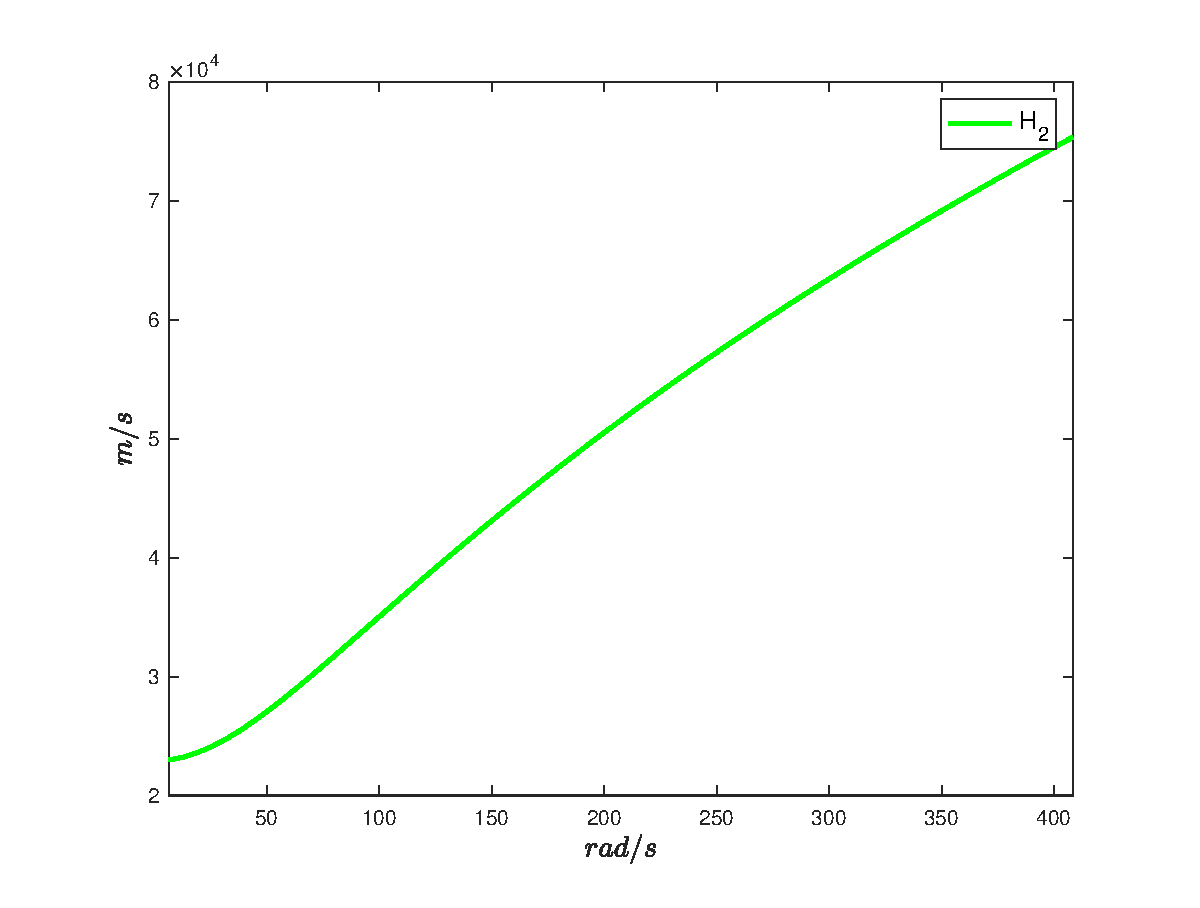
\includegraphics[scale=.42]{phase_velocity_eletromag_h2}}
%\subfloat{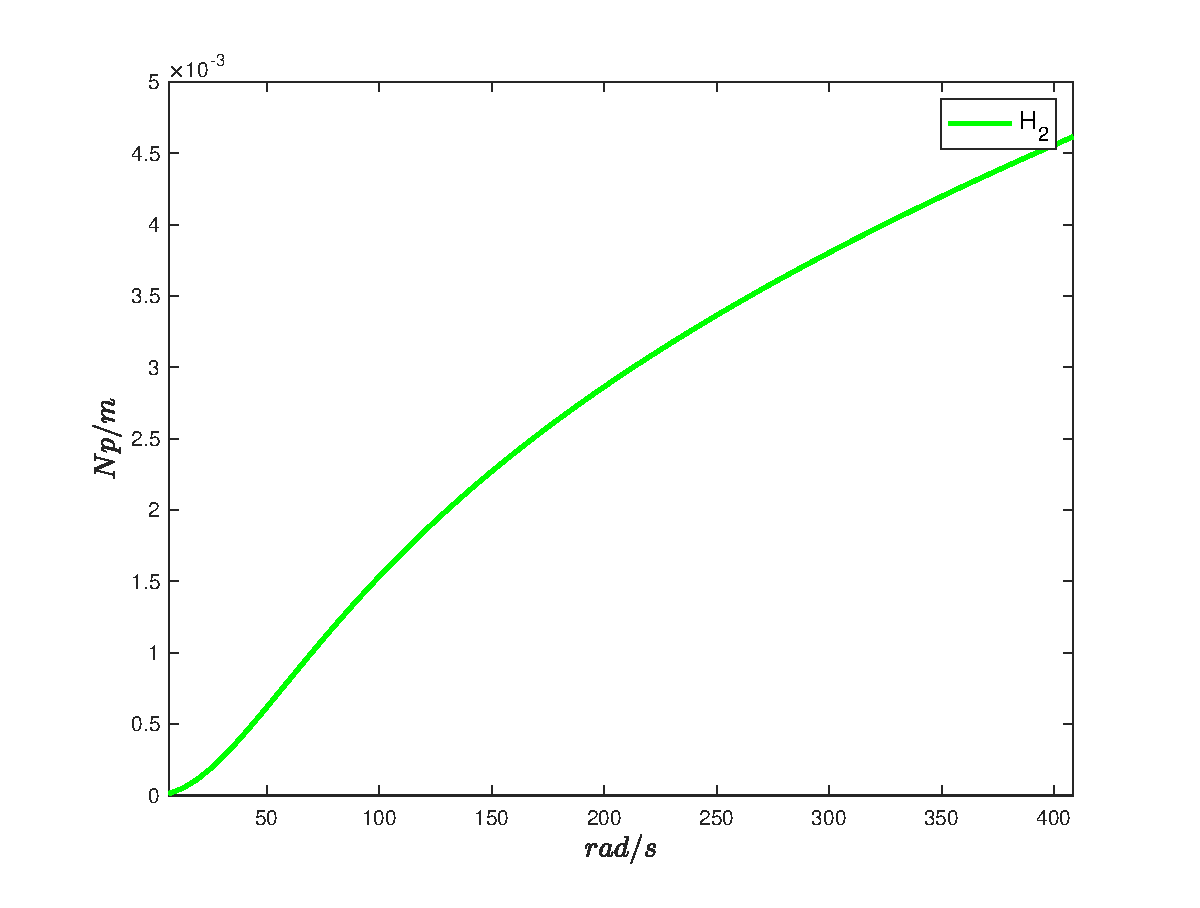
\includegraphics[scale=.42]{attenuation_eletromag_h2}}
\caption{\textit{Caso $V_H\neq0$, $H_1^0=0$ e $H_2^0=0$. Velocidade de fase e atenua\c{c}\~ao de duas ondas el\'asticas e de duas ondas eletromagn\'eticas, em fun\c{c}\~ao da frequ\^encia angular e do campo magn\'etico externo.}}
\label{fig.mag_horiz_ext_nula}
\end{figure}


\subsection{Subcaso $V_H=0$.}
Em meios com eletrocondutividade infinita temos a viscosidade magn\'etica igual a zero, e integrando as equa\c{c}\~oes (\ref{eq.H1_time}) e (\ref{eq.H2_time}) em rela\c{c}\~ao ao tempo, as mesmas passam a ser escritas na forma
\begin{align*}
H_1&=-H_1^0\frac{\partial u_3}{\partial z}+H_3^0\frac{\partial u_1}{\partial z}\\\\
H_2&=-H_2^0\frac{\partial u_3}{\partial z}+H_3^0\frac{\partial u_2}{\partial z}.
\end{align*}
Derivando as equa\c{c}\~oes acima em rela\c{c}\~ao a $z$ e substituindo-as nas equa\c{c}\~oes (\ref{eq.u1_time}), (\ref{eq.u2_time}) e (\ref{eq.u3_time}), temos que os campos el\'asticos n\~ao dependem mais das componentes eletromagn\'eticas, mas apenas do campo magn\'etico externo e dos par\^ametros eletromagn\'eticos e el\'asticos. Ou seja,
\begin{align*}
\rho\frac{\partial^2 u_1}{\partial t^2}&=-\mu_0H^0_1H^0_3\frac{\partial^2 u_3}{\partial z^2}+\left[G+\mu_0(H^0_3)^2\right]\frac{\partial^2 u_1}{\partial z^2}\\\\
\rho\frac{\partial^2 u_2}{\partial t^2}&=-\mu_0H^0_3H^0_2\frac{\partial^2 u_3}{\partial z^2}+\left[G+\mu_0(H^0_3)^2\right]\frac{\partial^2 u_2}{\partial z^2}\\\\
\rho\frac{\partial^2 u_3}{\partial t^2}&=\{(\lambda+2G)+\mu_0\left[(H^0_2)^2+(H^0_1)^2\right]\}\frac{\partial^2 u_3}{\partial z^2}-\mu_0H^0_3H^0_2\frac{\partial^2 u_2}{\partial z^2}-\mu_0H^0_1H^0_3\frac{\partial^2 u_1}{\partial z^2}.
\end{align*}
Aplicando as solu\c{c}\~oes em ondas planas, constru\'imos o sistema homog\^eneo
\begin{empheq}[left=\empheqlbrace]{align}\nonumber
&\{\left[G+\mu_0(H^0_3)^2\right]k^2-\rho\omega^2\}u_{01}-\mu_0H^0_1H^0_3k^2u_{03}=0\\\label{eq.slavas_system}
&\{\left[G+\mu_0(H^0_3)^2\right]k^2-\rho\omega^2\}u_{02}-\mu_0H^0_2H^0_3k^2u_{03}=0\\\nonumber
&\mu_0H^0_1H^0_3k^2u_{01}+\mu_0H^0_2H^0_3k^2u_{02}-\\\nonumber
&\qquad\{(\lambda+2G)k^2+\mu_0\left[(H^0_1)^2+(H^0_2)^2\right]k^2-\rho\omega^2\}u_{03}=0,
\end{empheq}
o qual nos permite analisar tr\^es situa\c{c}\~oes abaixo descritas.

\subsubsection{Condutividade infinita e $H_3^0=0$.}
Considerando $H_3^0=0$ no sistema (\ref{eq.slavas_system}), temos que a rela\c{c}\~ao de dispers\~ao para a componente $u_3$ \'e 
\begin{equation}
\{\lambda+2G+\mu_0\left[(H^0_1)^2+(H^0_2)^2\right]\}k^2-\rho\omega^2=0,
\end{equation}
de onde podemos isolar o n\'umero de onda
\begin{equation}
k=\omega\sqrt{\frac{\rho}{\lambda+2G+\mu_0\left[(H^0_1)^2+(H^0_2)^2\right]}},
\end{equation}
e extrair somente a velocidade de fase.
Note que, para esta componente, a velocidade n\~ao depende da frequ\^encia angular, depende apenas das primeiras componentes do campo magn\'etico externo, e podemos observar seu gr\'afico na figura (\ref{fig.mech_funcao_campo_ext}). Apesar da grande varia\c{c}\~ao do campo magn\'etico externo, entre 0 e $10^5\,T$, a velocidade se mant\'em praticamente constante.
Para as outras componentes temos a sequinte rela\c{c}\~ao de dispers\~ao onde a velocidade \'e constante e n\~ao depende do campo magn\'etico externo,
\begin{equation}
\left[G+\mu_0(H^0_3)^2\right]k^2-\rho\omega^2=0\quad\Rightarrow\quad k=\omega\sqrt{\frac{\rho}{G}}.
\end{equation} 
 

\subsubsection{Condutividade infinita, $H_1^0=0$ e $H_2^0=0$.}

Desprezando as componentes horizontais do campo magn\'etico externo no sistema (\ref{eq.slavas_system}), a velocidade de fase da terceira componente do campo el\'astico \'e constante, n\~ao dependendo da frequ\^encia nem da componente do campo externo remanescente,
\begin{equation}
k=\omega\sqrt{\frac{\rho}{\lambda+2G}}.
\end{equation}
A velocidade das demais componentes el\'asticas dependem apenas do campo magn\'etico externo, e o n\'umero de onda \'e dado por
\begin{equation}
k=\omega\sqrt{\frac{\rho}{G+\mu_0(H_3^0)^2}}.
\end{equation}
Os gr\'aficos tamb\'em podem ser observados na figura (\ref{fig.mech_funcao_campo_ext}), as velocidades se mant\^em praticamente constantes em fun\c{c}\~ao do campo externo e as atenua\c{c}\~oes s\~ao nulas.

\subsubsection{Condutividade infinita, $H_1^0\neq0$, $H_2^0\neq0$ e $H_3^0\neq0$.}

Para o caso com atua\c{c}\~ao das tr\^es componentes do campo magn\'etico externo, a rela\c{c}\~ao de dispers\~ao obtida do sistema (\ref{eq.slavas_system}) \'e dada por
\begin{empheq}[left=\empheqlbrace]{align}\nonumber
&\left[G+\mu_0(H^0_3)^2\right]k^2-\rho\omega^2=0\\\nonumber
&\{\left[G+\mu_0(H^0_3)^2\right]k^2-\rho\omega^2\}\left[-(\lambda+2G)k^2-\mu_0(H_1^0+H_2^0)k^2+\rho\omega^2\right]+\\\label{eq.sigma_inf_3}
&\qquad\qquad\qquad\qquad\qquad\qquad\qquad\quad\,\,\,\,\mu_0(H_3^0)^2\left[(H_1^0)^2+(H_2^0)^2\right]k^4=0.
\end{empheq}
A equa\c{c}\~ao (\ref{eq.sigma_inf_3}) pode ser resolvida com a abordagem da subse\c{c}\~ao (\ref{sec.dispesion_1D}),
%\begin{equation}
%a\,k^4+b\,\rho\,\omega^2k^2-\rho^2\omega^4=0,
%\end{equation}
%sendo 
%\begin{empheq}[left=\empheqlbrace]{align*}
%a&=[G+\mu_0(H^0_3)^2][-\lambda-2G-\mu_0(H^0_1+H^0_2)]+\mu_0(H^0_3)^2[(H^0_1)^2+(H^0_2)^2]\\
%b&=G+\mu_0(H^0_3)^2+\lambda+2G+\mu_0(H^0_1+H^0_2),
%\end{empheq}
%e suas ra\'izes s\~ao dadas por 
%\begin{equation}
%k=\omega\left(\frac{-b\rho\pm\rho\sqrt{b^2+4\,a}}{2\,a}\right)^{\frac{1}{2}}.
%\end{equation}
e para este \'ultimo subcaso, observamos que a velocidade de fase de qualquer campo el\'astico n\~ao depende da frequ\^encia angular, mas depende de todas as componentes do campo magn\'etico externo. 
% IF NEEDED, WE CAN BUILD THE GRAPHICS TO SHOW THE NULL ATTENUATION FOR THE WHOLE FREQUENCY DOMAIN.
Al\'em disso, temos que a atenua\c{c}\~ao das ondas mec\^anicas tamb\'em sob essas condi\c{c}\~oes \'e nula para todo o dom\'inio da frequ\^encia. A varia\c{c}\~ao da velocidade de fase em fun\c{c}\~ao do campo externo tamb\'em est\'a na figura (\ref{fig.mech_funcao_campo_ext}), e observe que para todos os tr\^es subcasos com viscosidade magn\'etica nula as velocidades das ondas mec\^anicas praticamente n\~ao sofrem influ\^encia do campo magn\'etico externo, apesar da curva apresentada no gr\'afico.

\begin{figure}
\centering
\subfloat{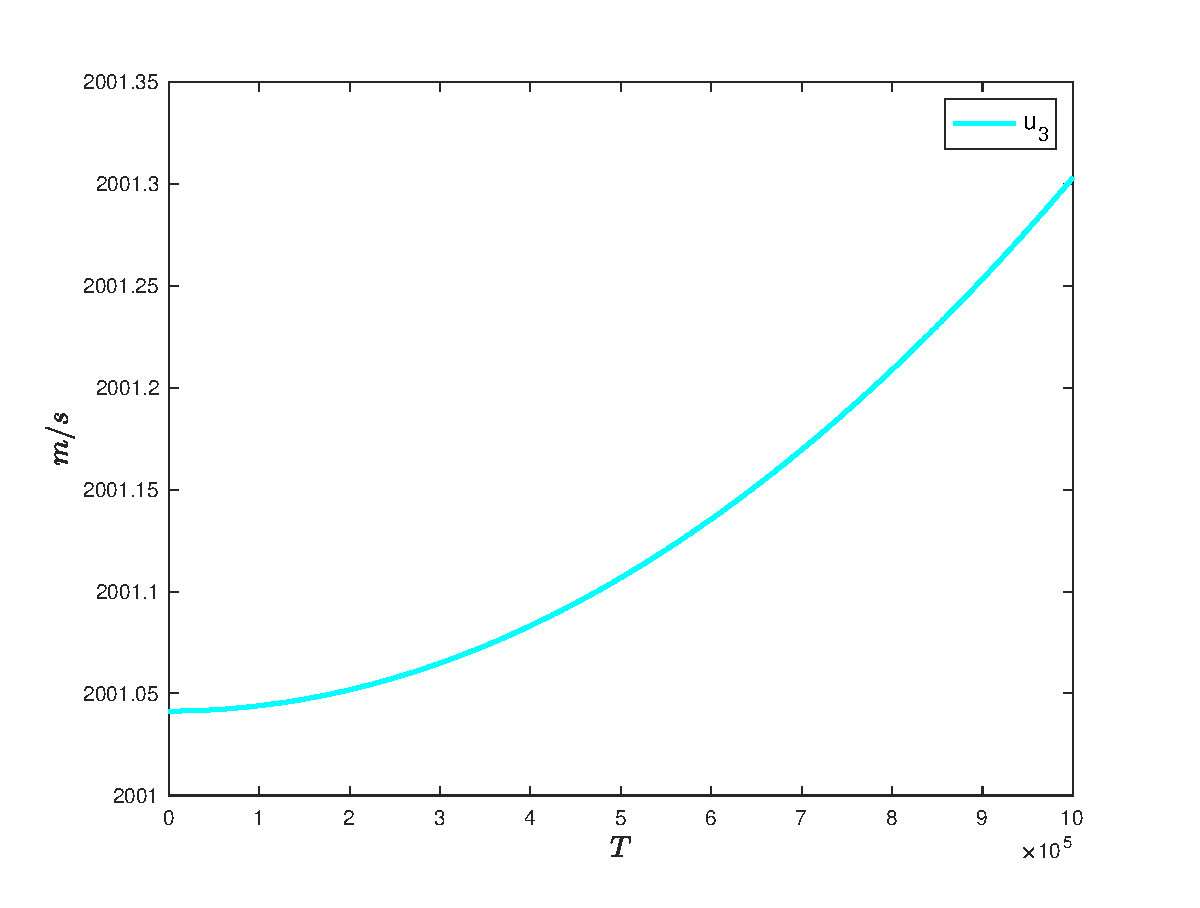
\includegraphics[scale=.43]{VH=0_0h3=0_phas_veloc}}
\subfloat{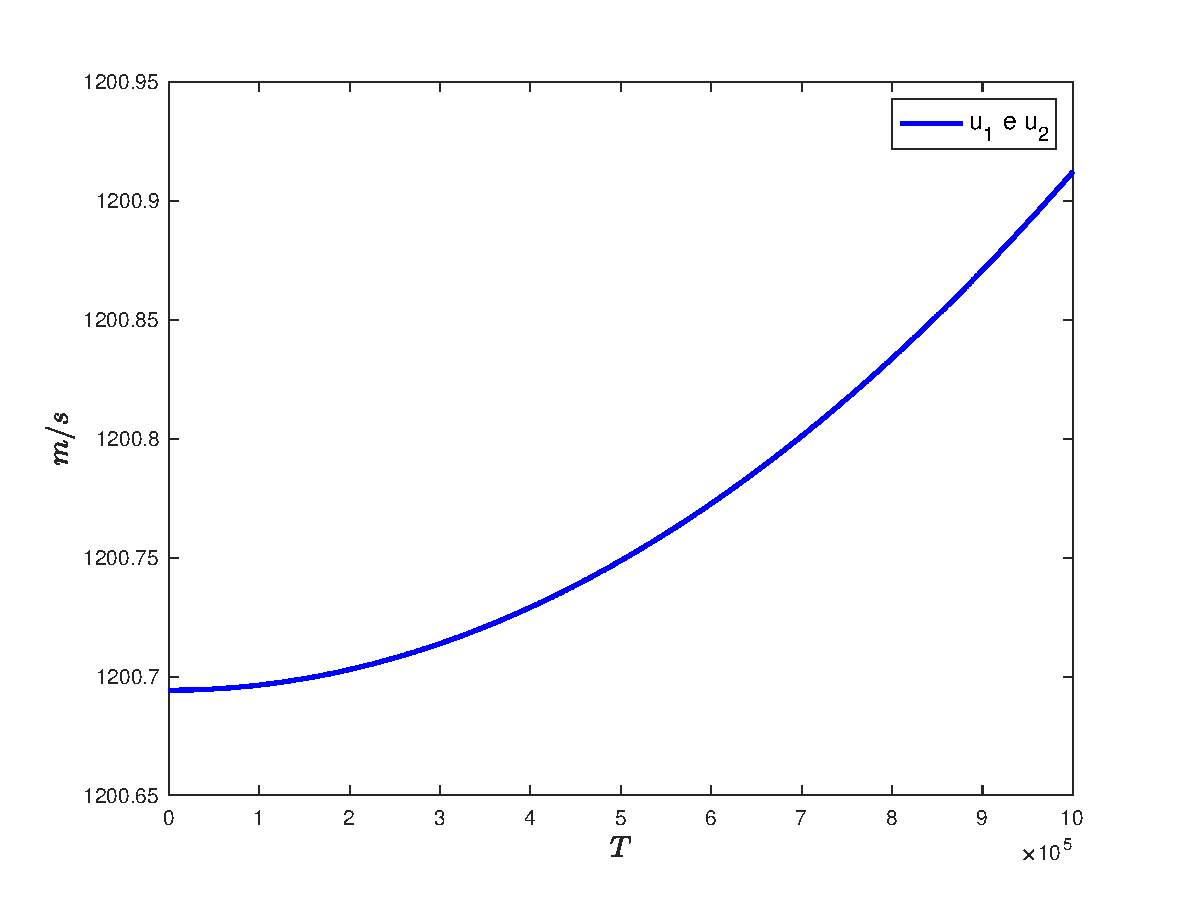
\includegraphics[scale=.43]{VH=0_0h1=0h2=0_phas_veloc}}\\
\subfloat{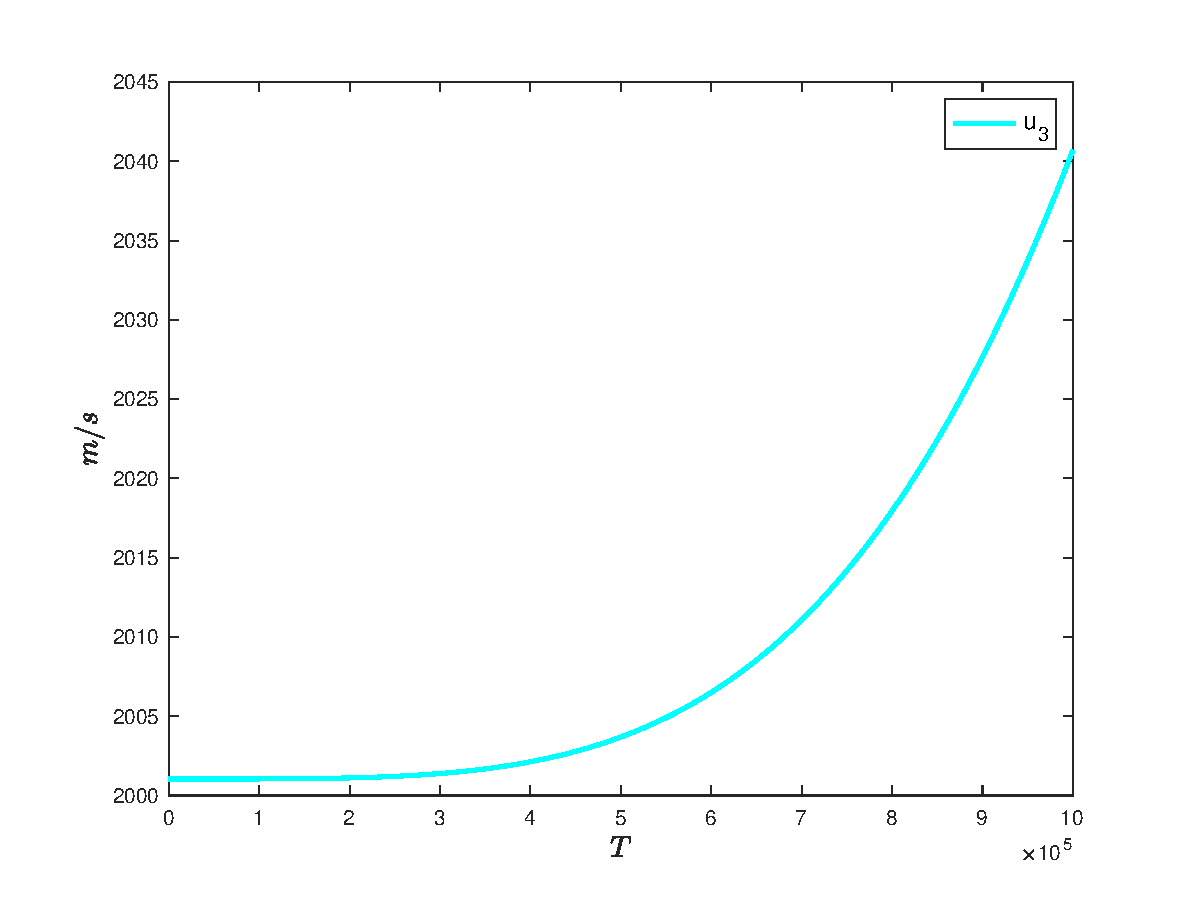
\includegraphics[scale=.43]{VH=0_all_external_null_u_3}}
\subfloat{\includegraphics[scale=.43]{VH=0_all_external_null_u1_u2}}
\caption{\textit{Considerando a condutividade infinita, a atenua\c{c}\~ao dos campos mec\^anicos \'e sempre nula. Em cima e \`a esquerda: $H^0_3=0$. Em cima e \`a direita: $H^0_1=H^0_2=0$. Embaixo: velocidade para as tr\^es componentes do campo externo n\~ao nulas. }}
\label{fig.mech_funcao_campo_ext}
\end{figure}

\section{An\'alise de Dispers\~ao e Atenua\c{c}\~ao de Ondas se Propagando em tr\^es Dimens\~oes}
Para efetuar a an\'alise de dispers\~ao e atenua\c{c}\~ao em seu caso mais geral usando os sistemas (\ref{eq.disp_abertas_1}) e (\ref{eq.disp_abertas_2}), vamos utilizar os procedimentos que podem ser encontrados  em \cite{sharma_08} e \cite{Blanc_13}, por exemplo. Sendo assim, escrevendo as solu\c{c}\~oes em termos de ondas planas, temos
\begin{equation}\label{eq.ondas_planas_3D}
\mathbf{\widehat{H}}=\mathbf{H}_0e^{-i(\omega\,t-\mathbf{k}\cdot\mathbf{x})}\qquad\text{e}\qquad \mathbf{\widehat{u}}=\mathbf{u}_0e^{-i(\omega\,t-\mathbf{k}\cdot\mathbf{x})},
\end{equation}
onde $\mathbf{H}_0$ e $\mathbf{u}_0$ s\~ao as polariza\c{c}\~oes e $\mathbf{k}$ \'e o vetor de onda.
Substituindo as solu\c{c}\~oes em ondas planas dadas pelas equa\c{c}\~oes \ref{eq.ondas_planas_3D} na equa\c{c}\~ao \ref{eq.disp_1}, avaliando as derivadas parciais e eliminando as exponenciais, temos
\begin{equation*}
\frac{\norm{\mathbf{k}}^2-(\sigma-i\,\epsilon\,\omega)\,i\,\omega\,\mu_0}{\omega\,\sigma\,\mu_0}\mathbf{H}_0-
\begin{pmatrix}
-H_3^0k_x-H_2^0k_y&H_1^0k_y&H_1^0k_x\\
H_2^0k_z&-H_1^0k_z-H_3^0k_x&H_2^0k_x\\
H_3^0k_z&H_3^0k_y&-H_2^0k_y-H_1^0k_z
\end{pmatrix}
\mathbf{u}_0
=0.
\end{equation*}
Procedendo analogamente para a equa\c{c}\~ao \ref{eq.disp_2}, temos
\begin{align*}
i\,\mu_0
\begin{pmatrix}
H_3^0k_z+H_2^0k_y&-H_2^0k_x&-H_3^0k_x\\
-H_1^0k_y&H_3^0k_z+H_1^0k_x&-H_3^0k_y\\
-H_1^0k_z&-H_2^0k_z&H_1^0k_x+H_2^0k_y
\end{pmatrix}
\mathbf{H}_0
&-\\\\
\begin{pmatrix}
\alpha_1&(\lambda+G)k_xk_y&(\lambda+G)k_xk_z\\
(\lambda+G)k_xk_y&\alpha_2&(\lambda+G)k_yk_z\\
(\lambda+G)k_xk_z&(\lambda+G)k_yk_z&\alpha_3
\end{pmatrix}
\mathbf{u}_0
&=0.
\end{align*}
onde 
\begin{empheq}[left=\empheqlbrace]{align*}
\alpha_1&=(\lambda+2\,G)k_x^2+G\,k_y^2+G\,k_z^2-\omega^2\rho\,\mu_0\\
\alpha_2&=(\lambda+2\,G)k_y^2+G\,k_x^2+G\,k_z^2-\omega^2\rho\,\mu_0\\
\alpha_3&=(\lambda+2\,G)k_z^2+G\,k_y^2+G\,k_x^2-\omega^2\rho\,\mu_0.
\end{empheq}
Usando as defini\c{c}\~oes de \cite{White_Zhou_2006} e \cite{sharma_08} para a vagarozidade de uma onda, temos, respectivamente,
\begin{equation*}
\mathbf{p}=\frac{1}{\omega}\mathbf{k}\qquad \text{e}\qquad \mathbf{p}=\frac{1}{V}\mathbf{N},
\end{equation*}
onde, utilizando a nota\c{c}\~ao em \cite{sharma_08}, $\mathbf{p}$ \'e a vagarozidade, $V$ \'e a velocidade de fase e $\mathbf{N}$ \'e a dire\c{c}\~ao de propaga\c{c}\~ao da onda. Assim, deduzimos que
\begin{equation}\label{eq.k_omega__veloc_fase}
\mathbf{k}=\frac{\omega}{V}\mathbf{N}.
\end{equation}
Observando que $\mathbf{N}$ \'e unit\'ario e substituindo a equa\c{c}\~ao \ref{eq.k_omega__veloc_fase} nas equa\c{c}\~oes matriciais acima, temos
\begin{equation*}
\frac{\frac{\omega}{V^2}-(\sigma-i\,\epsilon\,\omega)\,i\,\mu_0}{\sigma\,\mu_0}\mathbf{H}_0-\frac{\omega}{V}
\begin{pmatrix}
-H_3^0n_x-H_2^0n_y&H_1^0n_y&H_1^0n_x\\
H_2^0n_z&-H_1^0n_z-H_3^0n_x&H_2^0n_x\\
H_3^0n_z&H_3^0n_y&-H_2^0n_y-H_1^0n_z
\end{pmatrix}
\mathbf{u}_0
=0.
\end{equation*}
e
\begin{align*}
i\,\mu_0\frac{\omega}{V}
\begin{pmatrix}
H_3^0n_z+H_2^0n_y&-H_2^0n_x&-H_3^0n_x\\
-H_1^0n_y&H_3^0n_z+H_1^0n_x&-H_3^0n_y\\
-H_1^0n_z&-H_2^0n_z&H_1^0n_x+H_2^0n_y
\end{pmatrix}
\mathbf{H}_0
&-\\\\\ \frac{\omega^2}{V^2} 
\begin{pmatrix}
\alpha_1&(\lambda+G)n_xn_y&(\lambda+G)n_xn_z\\
(\lambda+G)n_xn_y&\alpha_2&(\lambda+G)n_yn_z\\
(\lambda+G)n_xn_z&(\lambda+G)n_yn_z&\alpha_3
\end{pmatrix}
\mathbf{u}_0
-\omega^2\rho\,\mu_0I_{3\times 3}\mathbf{u}_0
&=0.
\end{align*}
onde 
\begin{empheq}[left=\empheqlbrace]{align*}
\alpha_1&=(\lambda+2\,G)n_x^2+G\,n_y^2+G\,n_z^2\\
\alpha_2&=(\lambda+2\,G)n_y^2+G\,n_x^2+G\,n_z^2\\
\alpha_3&=(\lambda+2\,G)n_z^2+G\,n_y^2+G\,n_x^2.
\end{empheq}
Com a finalidade de facilitar a determina\c{c}\~ao da dire\c{c}\~ao de propaga\c{c}\~ao das ondas, vamos transferir a representa\c{c}\~ao do vetor dire\c{c}\~ao do espa\c{c}o em coordenadas cartesianas para coordenadas esf\'ericas. Lembrando que o vetor $\mathbf{N}$ que fornnece a dire\c{c}\~ao \'e um vetor normalizado e considerando a figura \ref{fig.frame_dispersao}, temos que as componentes de $\mathbf{N}$ em termos dos \^angulos $\phi$ e $\theta$ s\~ao
\begin{align*}
n_x&=\text{sen}\,\phi\,\cos\theta\\
n_y&=\text{sen}\,\phi\,\text{sen}\,\theta\\
n_z&=\cos\phi
\end{align*}
\begin{figure}
\centering
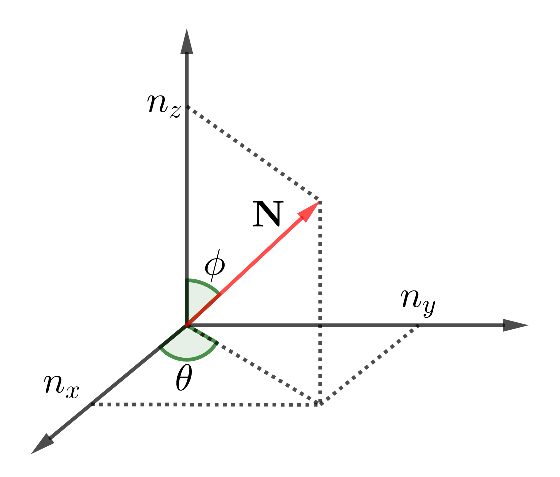
\includegraphics[scale=1]{frame_dispersao}
\caption{\textit{Convers\~ao do vetor de dire\c{c}\~ao de propaga\c{c}\~ao das fases de coordenadas cartesianas para coordenadas cil\'indricas.}}
\label{fig.frame_dispersao}
\end{figure}
Analogamente, vamos aplicar o campo magn\'etico externo em termos de suas magnitude e dire\c{c}\~ao, pois desse modo poderemos visualizar separadamente como cada uma dessas duas caracter\'isticas influenciam a dispers\~ao e atenua\c{c}\~ao de ondas el\'asticas. Com pequena diferen\c{c}a na nota\c{c}\~ao, a visualiza\c{c}\~ao para essa transforma\c{c}\~ao tamb\'em pode ser acompanhada pela figura  \ref{fig.frame_dispersao}. Sendo assim, temos
\begin{align*}
H_1^0&=H^0\text{sen}\,\phi^0\cos\theta^0\\
H_2^0&=H^0\text{sen}\,\phi^0\text{sen}\,\theta^0\\
H_3^0&=H^0\cos\phi^0,
\end{align*}
onde $H^0$ representa a magnitude do campo magn\'etico externo.

\begin{landscape}
Escrevevendo nossas equa\c{c}\~oes matriciais em termos dos \^angulos $\phi$ e $\theta$, temos
\begin{equation}\label{eq.matricial_disp_1}
\frac{\frac{\omega}{V^2}-(\sigma-i\,\epsilon\,\omega)\,i\,\mu_0}{\sigma\,\mu_0}\mathbf{H}_0-\frac{\omega}{V}
\begin{pmatrix}
-H_3^0\text{sen}\,\phi\,\cos\theta-H_2^0\text{sen}\,\phi\,\text{sen}\,\theta&H_1^0\text{sen}\,\phi\,\text{sen}\,\theta&H_1^0\text{sen}\,\phi\,\cos\theta\\
H_2^0\cos\phi&-H_1^0\cos\phi-H_3^0\text{sen}\,\phi\,\cos\theta&H_2^0\text{sen}\,\phi\,\cos\theta\\
H_3^0\cos\phi&H_3^0\text{sen}\,\phi\,\text{sen}\,\theta&-H_2^0\text{sen}\,\phi\,\text{sen}\,\theta-H_1^0\cos\phi
\end{pmatrix}
\mathbf{u}_0
=0.
\end{equation}
e
\begin{align}\nonumber
i\,\mu_0\frac{\omega}{V}
\begin{pmatrix}
H_3^0\cos\phi+H_2^0\text{sen}\,\phi\,\text{sen}\,\theta&-H_2^0\text{sen}\,\phi\,\cos\theta&-H_3^0\text{sen}\,\phi\,\cos\theta\\
-H_1^0\text{sen}\,\phi\,\text{sen}\,\theta&H_3^0\cos\phi+H_1^0\text{sen}\,\phi\,\cos\theta&-H_3^0\text{sen}\,\phi\,\text{sen}\,\theta\\
-H_1^0\cos\phi&-H_2^0\cos\phi&H_1^0\text{sen}\,\phi\,\cos\theta+H_2^0\text{sen}\,\phi\,\text{sen}\,\theta
\end{pmatrix}
\mathbf{H}_0
&-\\\label{eq.matricial_disp_2}\\\nonumber
\frac{\omega^2}{V^2} 
\begin{pmatrix}
\alpha_1&(\lambda+G)\text{sen}^2\,\phi\cos\theta\,\text{sen}\,\theta&(\lambda+G)\text{sen}\,\phi\,\cos\theta\,\cos\phi\\
(\lambda+G)\text{sen}^2\,\phi\,\cos\theta\,\text{sen}\,\theta&\alpha_2&(\lambda+G)\text{sen}\,\phi\,\text{sen}\,\theta\,\cos\phi\\
(\lambda+G)\text{sen}\,\phi\,\cos\theta\,\cos\phi&(\lambda+G)\text{sen}\,\phi\,\text{sen}\,\theta\,\cos\phi&\alpha_3
\end{pmatrix}
\mathbf{u}_0
-\omega^2\rho\,\mu_0I_{3\times 3}\mathbf{u}_0
&=0.
\end{align}
onde 
\begin{empheq}[left=\empheqlbrace]{align*}
\alpha_1&=(\lambda+2\,G)(\text{sen}\,\phi\,\cos\theta)^2+G\,(\text{sen}\,\phi\,\text{sen}\,\theta)^2+G\,\cos^2\phi\\
\alpha_2&=(\lambda+2\,G)(\text{sen}\,\phi\,\text{sen}\,\theta)^2+G\,(\text{sen}\,\phi\,\cos\theta)^2+G\,\cos^2\phi\\
\alpha_3&=(\lambda+2\,G)\cos^2\phi+G\,(\text{sen}\,\phi\,\text{sen}\,\theta)^2+G\,(\text{sen}\,\phi\,\cos\theta)^2.
\end{empheq}
Vamos isolar a solu\c{c}\~ao para o campo magn\'etico na equa\c{c}\~ao \ref{eq.matricial_disp_1}, obtendo 
\begin{equation}\label{eq.solucao_magnetico}
\mathbf{H}_0=\frac{\sigma\,\omega\,\mu_0}{V\,[\frac{\omega}{V}-(\sigma-i\,\epsilon\,\omega)\,i\,\mu_0]}
\begin{pmatrix}
-H_3^0\text{sen}\,\phi\,\cos\theta-H_2^0\text{sen}\,\phi\,\text{sen}\,\theta&H_1^0\text{sen}\,\phi\,\text{sen}\,\theta&H_1^0\text{sen}\,\phi\,\cos\theta\\
H_2^0\cos\phi&-H_1^0\cos\phi-H_3^0\text{sen}\,\phi\,\cos\theta&H_2^0\text{sen}\,\phi\,\cos\theta\\
H_3^0\cos\phi&H_3^0\text{sen}\,\phi\,\text{sen}\,\theta&-H_2^0\text{sen}\,\phi\,\text{sen}\,\theta-H_1^0\cos\phi
\end{pmatrix}
\mathbf{u}_0.
\end{equation}
Definimos
\begin{align*}
B&=
\begin{pmatrix}
-H_3^0\text{sen}\,\phi\,\cos\theta-H_2^0\text{sen}\,\phi\,\text{sen}\,\theta&H_1^0\text{sen}\,\phi\,\text{sen}\,\theta&H_1^0\text{sen}\,\phi\,\cos\theta\\
H_2^0\cos\phi&-H_1^0\cos\phi-H_3^0\text{sen}\,\phi\,\cos\theta&H_2^0\text{sen}\,\phi\,\cos\theta\\
H_3^0\cos\phi&H_3^0\text{sen}\,\phi\,\text{sen}\,\theta&-H_2^0\text{sen}\,\phi\,\text{sen}\,\theta-H_1^0\cos\phi
\end{pmatrix},\\\\
C&
=\begin{pmatrix}
H_3^0\cos\phi+H_2^0\text{sen}\,\phi\,\text{sen}\,\theta&-H_2^0\text{sen}\,\phi\,\cos\theta&-H_3^0\text{sen}\,\phi\,\cos\theta\\
-H_1^0\text{sen}\,\phi\,\text{sen}\,\theta&H_3^0\cos\phi+H_1^0\text{sen}\,\phi\,\cos\theta&-H_3^0\text{sen}\,\phi\,\text{sen}\,\theta\\
-H_1^0\cos\phi&-H_2^0\cos\phi&H_1^0\text{sen}\,\phi\,\cos\theta+H_2^0\text{sen}\,\phi\,\text{sen}\,\theta
\end{pmatrix}\quad\text{e}\\\\
D&=
\begin{pmatrix}
\alpha_1&(\lambda+G)\text{sen}^2\,\phi\cos\theta\,\text{sen}\,\theta&(\lambda+G)\text{sen}\,\phi\,\cos\theta\,\cos\phi\\
(\lambda+G)\text{sen}^2\,\phi\,\cos\theta\,\text{sen}\,\theta&\alpha_2&(\lambda+G)\text{sen}\,\phi\,\text{sen}\,\theta\,\cos\phi\\
(\lambda+G)\text{sen}\,\phi\,\cos\theta\,\cos\phi&(\lambda+G)\text{sen}\,\phi\,\text{sen}\,\theta\,\cos\phi&\alpha_3
\end{pmatrix}.
\end{align*}
Substituindo a express\~ao \ref{eq.solucao_magnetico} para o campo magn\'etico na equa\c{c}\~ao \ref{eq.matricial_disp_2} e usando as defini\c{c}\~oes acima, temos
\begin{equation}\label{eq.matricial_disp_3}
\frac{i\,\sigma\,\omega^2\mu^2}{V^2\,[\frac{\omega}{V}-(\sigma-i\,\epsilon\,\omega)\,i\,\mu_0]}
CB\,
\mathbf{u}_0
-\frac{\omega^2}{V^2}
D\,
\mathbf{u}_0
+\omega^2\rho\,\mu_0I=0.
\end{equation}
Eliminando o denominador, a equa\c{c}\~ao \ref{eq.matricial_disp_3} pode ser escrita como
\begin{equation}\label{eq.matricial_disp_4}
\begin{pmatrix}
i\,\sigma\,\mu_0^2(H^0)^2V^2CB+[(\sigma-i\,\epsilon\,\omega)\,i\,\mu_0V^2-\omega]\,D+[\omega\,\rho\,\mu_0V^2-(\sigma-i\,\epsilon\,\omega)\,i\,\rho\,\mu_0^2V^4]\,I
\end{pmatrix}
\mathbf{u}_0=0
\end{equation}
\end{landscape}
onde definimos
\begin{empheq}[left=\empheqlbrace]{align*}
a&=i\,\sigma\,\mu_0^2(H^0)^2\\
b&=(\sigma-i\,\epsilon\,\omega)\,i\,\mu_0\\
c&=\omega\,\rho\,\mu_0\\
d&=-(\sigma-i\,\epsilon\,\omega)\,i\,\rho\,\mu_0^2.
\end{empheq}
Para evitar a solu\c{c}\~ao n\~a	o trivial da equa\c{c}\~ao \ref{eq.matricial_disp_4}, precisamos garantir que 
\begin{equation}
det
\begin{pmatrix}
a\,V^2CB+[b\,V^2-\omega]\,D+[c\,V^2+d\,V^4]\,I
\end{pmatrix}
=0.
\end{equation}
A expans\~ao desse determinante nos fornece uma equa\c{c}\~ao onde podemos escrever a velocidade de fase em fun\c{c}\~ao da frequ\^encia angular, em fun\c{c}\~ao da dire\c{c}\~ao de propaga\c{c}\~ao das ondas mec\^anicas e em fun\c{c}\~ao da dire\c{c}\~ao de aplica\c{c}\~ao do campo magn\'etico externo. Assim, podemos realizar a an\'alise de dispers\~ao e atenua\c{c}\~ao de ondas el\'asticas no espa\c{c}o 3D.


